% HIER BITTE AUSFÜLLEN:

\newcommand{\abschlussarbeit}{Bachelorarbeit} % Bachelorarbeit / Masterarbeit
\newcommand{\zweitpruefer}{Prof. Dr. Guido Schryen} % Zweitprüfer

\newcommand{\sprache}{english} % Deutsch: german / Englisch: english
\newcommand{\druck}{oneside} %  / Simplex: oneside / Duplex: twoside

\newcommand{\titel}{Evaluating the Performance--Explainability Trade-off in Credit Scoring Under Regulatory Constraints}

\newcommand{\name}{Marius Calenborn}
\newcommand{\matrikelnummer}{7313033}
\newcommand{\adresse}{Ebbendorfer Straße 14, 49176 Hilter a.T.W.}
\newcommand{\upbmail}{mariusc@mail.uni-paderborn.de}
\newcommand{\abgabedatum}{19.08.2026}


% % % % % % % % % % % % % % % % % % % % % % % % % % % % % % % % % % % % % % %


\documentclass[fontsize=12pt,BCOR=15mm,DIV=15,a4paper,headsepline,headings=small,\druck,openany,appendixprefix]{scrbook}

\usepackage[onehalfspacing]{setspace}
\raggedbottom
\usepackage{emptypage}
\makeatother 
\usepackage{parskip}

\usepackage[utf8]{inputenc} % Zeichenkodierung
\usepackage[T1]{fontenc} % Trennung von Wörtern mit Umlauten
\usepackage{lmodern} % Latin Modern font benutzen (enhanced computer modern clone, serif)
\usepackage[\sprache]{babel} % Dokument in deutsch inklusive Silbentrennung nach neuer deutscher Rechtschreibung

\usepackage{amsmath} % verbesserte mathematische Umgebung
\usepackage{amsfonts} % zusätzliche mathematische Zeichen
\usepackage{amssymb} % zusätzliche mathematische Zeichen
\usepackage{amsthm} % zusätzliche mathematische Zeichen
\usepackage[hyphens]{url}
\usepackage{exscale} % Anpassung mathematischer Symbole an die Schriftgröße
\usepackage{amstext} % \text in mathematischer Umgebung
\usepackage{array} % Tabellen
\usepackage{rotating} % rotierte Tabellen und Bilder
\usepackage[algoruled, algochapter]{algorithm2e} % Pseudocode
\usepackage{verbatim} % Funktion zum Schreiben von unformatiertem Text
\usepackage[section]{placeins} % Verhindert das Wandern von floats in eine andere section
\usepackage{color} % Farbiger Text
\usepackage{graphicx} % Funktionen zum Einfügen von Bildern
\usepackage{subfigure} % Anzeigen von Bildern aus mehreren Einzelbildern
\usepackage[ngerman,\sprache]{babel}
\usepackage{setspace} % Einstellen des Zeilenabstandes
\usepackage[urlcolor = black,plainpages=false,pdfpagelabels=true,colorlinks=true,linkcolor=black,citecolor=black,bookmarksopen=true]{hyperref} % Verweise werden im PDF zu Hyperlinks
\usepackage[natbibapa]{apacite}
\usepackage{scrlayer-scrpage} % Koma für Kopfzeilen-Formatierung
\usepackage[nounderscore]{syntax}
\usepackage{tabulary} % bessere Tabellen
\usepackage{tabularx} % bessere Tabellen
\usepackage{longtable} % für Tabellen über mehrere Seiten
\usepackage{array}
\usepackage{paralist} % für kleine Einzüge mit \setdefaultleftmargin{0.5em}{}{}{}{}{}
\usepackage{booktabs}
\usepackage{multirow}
\usepackage[table,xcdraw]{xcolor}
\usepackage[hang]{footmisc} %Große Zahlen in Fußnoten
\makeatletter
\def\@makefnmark{\hbox{\textsuperscript\@thefnmark}}
% \ohead{\leftmark} %Only chapter in header (not section!)
\makeatother
\let\footnotesize\small

%\bibliographystyle{apalike} % Literaturverzeichnis entsprechend DIN 1505 formatiert, allerdings ohne URL und ISBN
\renewcommand{\topfraction}{0.85} % Anteil einer Seite, die von Floats belegt sein darf (default 0.7)
\renewcommand{\textfraction}{0.1} % Anteil einer Seite, die mindestens Text sein muss (default 0.2)
\renewcommand{\floatpagefraction}{0.75} % Anteil einer Seite, die ein Float einnehmen darf, ohne auf die nächste Seite gesetzt zu werden (default 0.5)



\usepackage{lipsum}

% Begin
\begin{document}

% Front Matter
\pagestyle{empty}
\pagenumbering{alph}

\input{title} 
\cleardoublepage

% Hilfsbefehl: Wert linksbündig auf der Linie, kleine Beschriftung darunter
\newcommand{\fillline}[3]{%
  \begin{minipage}[b]{#1}%
    \raggedright
    \underline{\makebox[\linewidth][l]{\strut #2}}\\[1pt]
    {\scriptsize #3}%
  \end{minipage}%
}

\noindent
\section*{Selbstständigkeitserklärung}

\noindent
{\small für die Abgabe von Bachelor-, Master-, Studien- und Hausarbeiten (§~63 Absatz~5 HG)}

% Name / Vorname und Matrikelnummer werden automatisch eingefügt
\noindent
\fillline{0.60\textwidth}{\textbf{\name}}{Vorname Nachname}%
\hfill
\fillline{0.35\textwidth}{\textbf{\matrikelnummer}}{Matrikelnummer}

\noindent
{\small Hiermit versichere ich, dass ich meine Bachelorarbeit mit dem Titel}

% Titel wird automatisch eingefügt; harte Umbrüche (\\) im Titel werden hier
% ignoriert, der Titel bricht nur bei Bedarf automatisch um
\noindent
\begin{minipage}[b]{\textwidth}
    \raggedright
    {\renewcommand{\\}{}\textbf{\titel\strut}}\par
    \rule{\linewidth}{0.2pt}
\end{minipage}


\noindent
{\small– bei einer Gruppenarbeit den entsprechend gekennzeichneten Teil der Arbeit – selbstständig verfasst und keine anderen als die angegebenen Quellen und Hilfsmittel benutzt habe.

\noindent
Die Stellen der Arbeit, die ich anderen Werken dem Wortlaut oder dem Sinn nach entnommen habe, habe ich in jedem Fall unter Angabe der Quellen entsprechend der wissenschaftlichen Standards sowohl an den Stellen im Text als auch im Literaturverzeichnis kenntlich gemacht. Das Gleiche gilt auch für Tabellen, Skizzen, Zeichnungen, bildliche Darstellungen usw.

\noindent
Sofern ich bei der Erstellung der Arbeit KI-generierte Inhalte (Text, Darstellungen, Programmcode etc.) verwendet habe, habe ich den Einsatz der KI-Tools sachgerecht dokumentiert und transparent gekennzeichnet. Hierbei habe ich mich an die Vorgaben der Prüfenden (siehe ``Erklärung über den Einsatz von Künstlicher Intelligenz'') gehalten.

\noindent
Mir ist bekannt, dass die ungekennzeichnete oder nicht angemessen gekennzeichnete Übernahme von fremdem geistigem Eigentum unabhängig von dessen Herkunft (auch aus dem Internet) oder die ungekennzeichnete oder nicht angemessen gekennzeichnete Übernahme von KI-generierten Texten eine Täuschung darstellen kann, die zur Folge hat, dass die Arbeit als mit der Note \quotedblbase mangelhaft\textquotedblleft{} (5,0) bewertet gilt. Dies umfasst auch die ungekennzeichnete oder nicht angemessen gekennzeichnete Übernahme von über das Allgemeinwissen hinausgehenden Fakten, Ideen, Argumenten oder spezifischen Formulierungen sowie deren Paraphrasierung oder Übersetzung.

\noindent
Ich habe die Arbeit nicht, auch nicht auszugsweise, für eine andere abgeschlossene Prüfung angefertigt.}

\medskip

% Ort und Datum wird automatisch eingefügt
\noindent
\fillline{0.55\textwidth}{\textbf{Paderborn, \abgabedatum}}{Ort und Datum}%
\hfill
\fillline{0.40\textwidth}{}{Unterschrift}

\noindent
{\tiny Selbstständigkeitserklärung \textperiodcentered{} Stand: November 2025}

\noindent
\section*{Erklärung über den Einsatz von Künstlicher Intelligenz}

Zur Erstellung dieser Arbeit wurde Künstliche Intelligenz eingesetzt.
Der Inhalt wurde anschließend überprüft, überarbeitet und die Verantwortung dafür liegt vollständig bei mir. Tabelle \ref{tab:ki_nutzung} zeigt, welche Arbeitsschritte mithilfe von KI‑Tools unterstützt wurden, welche Tools dabei zum Einsatz kamen und zu welchem Zweck sie genutzt wurden.

% #####
% Weitere Informationen zum Ausfüllen der Tabelle finden Sie unter:
% https://www.uni-paderborn.de/fileadmin/lehre/Handreichung_zur_Dokumentation_und_Kennzeichnung_von_KI-Tools.pdf
% #####

\bigskip

\begin{table}[h]
\centering
\begin{tabular}{|>{\raggedright\arraybackslash}m{3.5cm}|>{\raggedright\arraybackslash}m{4cm}|>{\raggedright\arraybackslash}m{6.5cm}|}
\hline
\centering\textbf{Arbeitsschritt}\arraybackslash &
\centering\textbf{Tool}\arraybackslash &
\centering\textbf{Verwendung}\arraybackslash \\
\hline
Konzeption & Claude (Anthropic)\newline ChatGPT (OpenAI)\newline Gemini (Google) & Diskussion, Konzeption und Strukturierung des Forschungsdesigns.\\
\hline
Einleitung & ChatGPT (OpenAI)\newline Claude (Anthropic) & Entwurf und sprachliche Überarbeitung englischer Textpassagen der Einleitung.\\
\hline
Literaturrecherche & NotebookLM (Google) & Zusammenfassung und Strukturierung vorhandener Quellen sowie Identifikation potenziell geeigneter weiterer Literatur auf deren Grundlage. \\
\hline
Endkorrektur & Claude (Anthropic)\newline ChatGPT (OpenAI)\newline Gemini (Google) & Prüfung auf sprachliche Korrektheit, Konsistenz und Struktur.\\
\hline
Programmieren & Claude Code (Anthropic) & Unterstützung bei der Python-Programmierung von Notebooks, Pipelines sowie Auswertungs- und Plot-Skripten. \\
\hline
Sonstiges & ChatGPT (OpenAI)\newline Claude (Anthropic) & Sprachliche Überarbeitung weiterer englischer Textpassagen sowie Unterstützung beim LaTeX-Satz (Tabellen, Grafiken und Formatierung).\\
\hline
\end{tabular}
\caption{Verwendung von Künstlicher Intelligenz in der Arbeit}
\label{tab:ki_nutzung}
\end{table}

\bigskip

Paderborn, \abgabedatum

\begin{flushright}
\bigskip
\bigskip
\bigskip

---------------------------------------------\\
\name
\end{flushright}



\bigskip

\cleardoublepage

\section*{Abstract -- English}

Credit scoring involves a potential trade-off between predictive performance and model explainability. Flexible boosted-tree ensembles can capture complex relationships but require post-hoc explanations, whereas intrinsically interpretable models expose their fitted prediction functions more directly. This thesis examines whether this structural difference is accompanied by a consistent performance disadvantage and what the findings show for model choice in the EU regulatory context.

Logistic regression and the Explainable Boosting Machine (EBM) were compared with XGBoost and CatBoost across four public credit datasets. The evaluation considered predictive and profit-based performance, supplemented by the stability and agreement of global feature rankings. Additional analyses examined whether the recorded patterns changed with training-set size or under chronological evaluation.

The results showed no uniform performance disadvantage for the EBM. A predictive and economic advantage for the boosted ensembles emerged on Lending Club, but this pattern did not recur across the other datasets. Profit-based results broadly reinforced the predictive comparison. The explanation analysis also showed no consistent stability advantage for the intrinsically interpretable models, although the EBM and the boosted ensembles frequently prioritised similar features. The additional analyses indicated that the magnitude of the differences varied across empirical settings, while the central Lending Club ordering remained unchanged under temporal validation.

These findings establish neither equivalence between model families nor regulatory compliance. They support evaluating functionally flexible glass-box models such as the EBM as primary candidates alongside boosted ensembles rather than treating them solely as transparency-oriented alternatives. Regulatory conformity ultimately depends on the complete deployed system rather than on model architecture alone.

\textbf{Keywords:} credit scoring, explainable AI, Explainable Boosting Machine, Expected Maximum Profit, EU AI Act


\begin{otherlanguage}{ngerman}

\section*{Abstrakt -- Deutsch}

Bei der Kreditwürdigkeitsprüfung besteht ein potenzieller Zielkonflikt zwischen Vorhersageleistung und Erklärbarkeit. Flexible Boosted-Tree-Ensembles können komplexe Zusammenhänge abbilden, benötigen jedoch nachgelagerte Erklärungsverfahren. Intrinsisch interpretierbare Modelle legen ihre gelernte Vorhersagefunktion dagegen unmittelbar offen. Diese Arbeit untersucht, ob dieser strukturelle Unterschied mit einem konsistenten Leistungsnachteil einhergeht und welche Bedeutung die Ergebnisse für die Modellauswahl im regulatorischen Kontext der Europäischen Union haben.

Hierzu wurden die logistische Regression und die Explainable Boosting Machine (EBM) mit XGBoost und CatBoost auf vier öffentlich verfügbaren Kreditdatensätzen verglichen. Die Evaluation berücksichtigte die prädiktive und gewinnorientierte Leistung, ergänzt um die Stabilität und Übereinstimmung globaler Merkmalsrangfolgen. Zusätzliche Analysen untersuchten, ob sich die beobachteten Muster mit zunehmender Größe der Trainingsdaten oder bei zeitlich getrennter Validierung veränderten.

Die Ergebnisse zeigten keinen konsistenten Leistungsnachteil für die EBM. Im Lending-Club-Datensatz ergab sich ein prädiktiver und wirtschaftlicher Vorteil für die Boosted-Tree-Ensembles, der sich auf den übrigen Datensätzen jedoch nicht konsistent wiederholte. Die gewinnorientierte Evaluation bestätigte weitgehend die Muster des prädiktiven Vergleichs. Auch bei der Stabilität der Merkmalsrangfolgen zeigte sich kein konsistenter Vorteil der intrinsisch interpretierbaren Modelle, obwohl die EBM und die Ensembles häufig ähnliche Merkmale priorisierten. Die zusätzlichen Analysen zeigten, dass die Größe der Unterschiede von den jeweiligen Untersuchungsbedingungen abhing, während die Modellreihenfolge auf Lending Club auch bei der zeitlichen Validierung erhalten blieb.

Die Befunde belegen weder eine exakte Gleichwertigkeit der Modellfamilien noch eine regulatorische Konformität. Sie sprechen aber dafür, funktional flexible Glass-Box-Modelle wie die EBM von Beginn an neben Boosted-Tree-Ensembles als eigenständige Modellkandidaten zu evaluieren und nicht lediglich als transparenzorientierte Alternative zu behandeln. Die regulatorische Konformität muss letztlich auf Ebene des gesamten eingesetzten Systems und nicht allein anhand der Modellarchitektur beurteilt werden.

\textbf{Stichworte:} Kreditwürdigkeitsprüfung, erklärbare künstliche Intelligenz, Explainable Boosting Machine, Attributionsstabilität, Expected Maximum Profit, EU AI Act


\end{otherlanguage}


\cleardoublepage

\pagestyle{scrheadings}
\clearscrheadfoot
\ohead{\headmark}
\ofoot{\pagemark}

\frontmatter

\tableofcontents
\cleardoublepage

\listoffigures
\cleardoublepage

\listoftables
\cleardoublepage

% Thesis
\mainmatter
\chapter{Introduction}

\section{Motivation}

Credit scoring is a consequential application of statistical and machine-learning
models in the financial sector: scoring outcomes can influence access to loans and
the conditions under which credit is offered, thus affecting an important dimension
of economic participation
\citep{bahloolPerformanceFairnessExplainability2026}. Model choice in this context
involves a tension. Flexible boosted-tree ensembles can represent nonlinear
relationships and interactions, but their fitted decision logic is not directly
inspectable and is therefore commonly explained post hoc. Inherently interpretable
models expose their decision structure more directly, but are often assumed to
sacrifice predictive performance
\citep{rudinStopExplainingBlack2019a, dessainCostExplainabilityAI2023}.

A recent systematic literature review questions how firmly this presumed trade-off is
established. It finds that predictive performance and explainability in AI-based credit
scoring are frequently assessed separately and that the
performance--explainability trade-off is more often assumed than directly quantified
\citep{bahloolPerformanceFairnessExplainability2026}. Existing direct comparisons
indicate that differences between interpretable and black-box models can be small and
depend on the dataset, preprocessing and model specification. Greater complexity
therefore does not necessarily produce a substantial predictive advantage
\citep{dessainCostExplainabilityAI2023,
amekoeExploringAccuracyInterpretability2024b}.

This issue also has regulatory relevance in the European Union. Under
Article~6(2) and Annex~III(5)(b) of Regulation~(EU)~2024/1689, creditworthiness
assessment is listed among the high-risk use cases for systems that fall within the
Act's definition of AI. The Act prescribes no model family but establishes requirements
concerning risk management, documentation, transparency, accuracy and human oversight
for covered high-risk systems. The GDPR applies independently where personal data are
processed and provides additional safeguards concerning certain automated individual
decisions \citep{mullerAIbasedCreditScoring2025, EUAIAct2024}.

To examine whether boosted-tree ensembles provide a consistent predictive or
profit-based advantage, this thesis compares two intrinsically interpretable models,
logistic regression (LR) and the Explainable Boosting Machine (EBM), with the
post-hoc-explained XGBoost and CatBoost ensembles. The EBM provides the central
glass-box case because it retains an additive, directly inspectable structure while
representing nonlinear effects and selected pairwise interactions
\citep{louAccurateIntelligibleModels2013,
noriInterpretMLUnifiedFramework2019}. Using two boosted-tree implementations also
examines whether recorded patterns recur within that model family.

Predictive performance and Expected Maximum Profit (EMP)
\citep{verbrakenDevelopmentApplicationConsumer2014} form the primary empirical
dimensions. Attribution-ranking stability and cross-model agreement provide supplementary
evidence on the resulting global explanation outputs, covering the reproducibility
and convergence of those outputs.

\section{Research Question and Objectives}\label{sec:rq}

The central research question is: \textit{Under the empirical conditions studied,
how do intrinsically interpretable credit-scoring models, particularly the EBM,
compare with post-hoc-explained boosted-tree ensembles in predictive and profit-based
performance, and what do the observed differences imply for model choice in the EU
regulatory context?}

The question is addressed in three empirical steps. First, the four pipelines are
compared across four public credit datasets in discrimination, classification performance and EMP. Second, the case-sampling stability
and cross-model agreement of their global source-feature attribution rankings are
examined. Third, training-size sensitivity is evaluated on Home Credit and Lending
Club, supplemented by out-of-time validation concerning Lending Club. The regulatory component situates these outcomes within the requirements that apply
to credit scoring under EU law, establishing what the empirical evidence can
contribute to a system-level assessment that reaches beyond model architecture. 

Chapter~\ref{ch:background} develops the conceptual, methodological and regulatory
background and derives the research gap from prior work, and
Chapter~\ref{ch:method} specifies the datasets, the four pipelines, the evaluation
measures and the prespecified analysis plan. Chapter~\ref{ch:results} reports the
performance, attribution and sensitivity results, Chapter~\ref{ch:discussion}
interprets them and states the limitations of the design, and
Chapter~\ref{ch:conclusion} answers the research question.

\chapter{Theoretical Background and Related Work}\label{ch:background}

\section{Conceptual and Regulatory Background}

\subsection{Credit Scoring Models and Interpretability}

Credit scoring is the task of estimating the probability that a borrower will
default, framed here as a binary classification problem \citep{lessmannBenchmarkingStateoftheartClassification2015}. Models
are grouped in this thesis by a structural criterion: whether the fitted object can
be read directly, or whether a second computation is needed to say what it does. The
criterion concerns the availability of an explanation, not its quality. An
intrinsically interpretable model with hundreds of correlated or transformed features
can be hard to grasp.

Logistic regression satisfies the criterion structurally because its coefficients
determine the prediction directly
\citep{liptonMythosModelInterpretability2018}. Their interpretation nevertheless
depends on feature scaling, categorical coding and the correlation structure, and
they act on the log-odds rather than directly on the probability.

The EBM provides a non-linear yet component-wise readable \emph{glass-box}
alternative. It is a generalised additive model extended by a limited number of
pairwise interactions, a GA\textsuperscript{2}M in the lineage of
\citet{louAccurateIntelligibleModels2013} and
\citet{noriInterpretMLUnifiedFramework2019}. It breaks down the link-transformed
expectation of default into
\begin{equation}
g\!\left(\mathbb{E}[y \mid x]\right) \;=\; \beta_0 \;+\; \sum_{j} f_j(x_j)
\;+\!\! \sum_{(j,k)\,\in\,\mathcal{I}} \!\! f_{jk}(x_j, x_k),
\label{eq:ebm}
\end{equation}
where $g$ is the link function, the logit here, so that the terms act on the log-odds
as in logistic regression. Each $f_j$ is a piecewise constant step function over the
binned values of feature~$j$, and $\mathcal{I}$ is the set of selected
interaction terms. Every term can
be plotted and read off exactly, in the sense that the terms reproduce the model
output rather than approximate it. They describe learned associations, not causal
effects \citep{amekoeExploringAccuracyInterpretability2024b}.

Gradient-boosted tree ensembles are constructed the other way round, building shallow
trees in stages, each fitted to the \emph{negative} gradient of the loss with respect to
the current ensemble prediction, the pseudo-residuals \citep{friedmanGreedyFunctionApproximation2001}. XGBoost \citep{chenXGBoostScalableTree2016} adds penalties on
leaf weights and tree complexity; CatBoost \citep{prokhorenkovaCatBoostUnbiasedBoosting2018} grows symmetric
trees and offers ordered target statistics for categorical variables. A single such
tree would be readable, an
ensemble of several hundred is not, because the decision logic is distributed across
them. An attribution method must therefore be applied on top \citep{zouInterpretableCreditScoring2025}.

This thesis accordingly distinguishes intrinsic explanations, read directly from the
fitted logistic regression and EBM, from post-hoc attributions computed for XGBoost and
CatBoost.



\subsection{Profit-Based Evaluation}\label{sec:emp}

ROC-AUC evaluates how well a model ranks applicants but does not capture
the asymmetric economic consequences of lending decisions. Rejecting an
applicant who would repay forfeits the return on the loan, whereas granting
credit to an applicant who defaults causes a loss on the principal.
Cost-sensitive measures incorporate these consequences but require economic
parameters that are rarely known with certainty and may affect the resulting
ranking of models
\citep{verbrakenDevelopmentApplicationConsumer2014}.

The Expected Maximum Profit (EMP) measure accounts for this uncertainty by
averaging the maximum attainable return over a distribution of loss severities.
\citet{verbrakenNovelProfitMaximizing2013a} introduce the general framework,
which \citet{verbrakenDevelopmentApplicationConsumer2014} adapt to consumer
credit scoring. Let $\pi_D$ and $\pi_N$ denote the proportions of defaulters
and non-defaulters, and let $R_D(t)$ and $R_N(t)$ denote the respective
fractions rejected at cut-off $t$. The loss fraction associated with a default
is $\lambda$, the loss given default expressed as a fraction of the principal.
The return forgone by rejecting a non-defaulting applicant is represented by
$\mathrm{ROI}$. Profit per applicant and per unit of principal is therefore

\begin{equation}
P(t;\lambda,\mathrm{ROI})
= \lambda\,\pi_D R_D(t)
- \mathrm{ROI}\,\pi_N R_N(t).
\label{eq:profit}
\end{equation}

Profit is measured relative to granting all applications. Rejecting nobody
sets both rejection rates to zero; because this policy remains available,
the maximised profit cannot be negative.

Rather than fixing $\lambda$ at a single value, EMP integrates the maximum
attainable return over its mixed distribution $H$:

\begin{equation}
\mathrm{EMP}
= \int_{[0,1]}
P\bigl(t^*(\lambda);\lambda,\mathrm{ROI}\bigr)\,
\mathrm{d}H(\lambda),
\qquad
t^*(\lambda)
= \arg\max_t P(t;\lambda,\mathrm{ROI}).
\label{eq:emp}
\end{equation}

The loss-given-default distribution and the assumed return are specified in the
empirical design. EMP remains conditional on these assumptions and on the class
prevalence and should not be interpreted as realised portfolio profit. Absolute EMP
values are therefore compared between models within one dataset rather than across
datasets.

\subsection{Explainability in Machine Learning}\label{sec:xai}

Explainability methods are commonly organised along two axes: whether an
explanation is \emph{inherent} to the model or produced \emph{post hoc}, and
whether it is \emph{global} (describing the whole model) or \emph{local}
(describing a single decision) \citep{nautaAnecdotalEvidenceQuantitative2023}. \citet{liptonMythosModelInterpretability2018} further
decomposes interpretability into simulatability, decomposability and algorithmic
transparency, and stresses that a post-hoc explanation is not the same as
transparency. 

Additive feature contributions provide a common representation over the four
evaluated pipelines. \citet{lundbergUnifiedApproachInterpreting2017} derive SHapley Additive exPlanations (SHAP) from the Shapley value in cooperative game theory:
features are treated as players, the prediction as the payout, and each attribution
as a feature's average marginal contribution across feature coalitions. The resulting
explanation is additive: the attributions and a base value reconstruct the prediction.
Within the class of additive feature-attribution methods, Shapley values uniquely
satisfy local accuracy, missingness and consistency.

Several limitations qualify what such an attribution establishes. It describes the
\emph{model}, not the world: a large attribution indicates that the fitted model relies
on a feature, not that the feature causes default
\citep{rudinStopExplainingBlack2019a,
liptonMythosModelInterpretability2018}. Attributions are also defined relative to a
reference distribution, so the same prediction can receive different attributions
under different references
\citep{nautaAnecdotalEvidenceQuantitative2023}. With correlated features, the
allocation of attribution among them additionally depends on the assumed dependence
structure \citep{aasExplainingIndividualPredictions2021}.

Two quantitative properties recur in this literature: \emph{stability}, the
reproducibility of explanations under resampling or retraining, and
\emph{faithfulness}, the extent to which an explanation accurately reflects the
behaviour of the fitted model
\citep{nautaAnecdotalEvidenceQuantitative2023}.

Separately from these properties of individual attribution procedures,
\citet{rudinStopExplainingBlack2019a} argues that high-stakes settings should prefer
inherently interpretable models over black boxes explained post hoc. This is a
structural argument about the relation between the model and its explanation, but it does
not establish that every post-hoc attribution is numerically inaccurate or that every
intrinsically interpretable model is readily understandable.

\subsection{Regulatory Framework}\label{sec:regulatory}

Credit scoring in the European Union is governed principally by the AI Act and the
GDPR \citep{mullerAIbasedCreditScoring2025}. The AI Act
(Regulation~(EU)~2024/1689) first requires a system to fall within the definition of
an AI system under Article~3(1) \citep{EUAIAct2024}. Whether conventional statistical
scorecards satisfy that definition remains relevant: the Commission guidance
discussed by \citet{mullerAIbasedCreditScoring2025} treats well-established linear and
logistic regression as outside the definition, but the guidance is not legally
binding.

Assuming that a deployed scoring system falls within Article~3(1),
creditworthiness assessment is listed in Annex~III(5)(b). Because the use considered
here profiles natural persons and materially informs the credit decision, the
derogation in Article~6(3) would not apply. The classification therefore depends on
the system along with its intended use rather than on the selected model family.

For covered high-risk systems, the Act allocates obligations between providers and
deployers. Article~13 specifies transparency plus information requirements for the
system and its instructions for use, while Article~16(a) requires the provider to
ensure that these requirements are met. Article~15 requires an appropriate level of
accuracy and robustness. Article~86 provides a right to an explanation against the
deployer only under its statutory conditions: the decision must be based on the
system's output and adversely affect the person in a legally or similarly significant
way, and the right applies only insofar as it does not already follow from other Union
law. GDPR Article~15(1)(h), by contrast, concerns the controller \citep{EUAIAct2024, mullerAIbasedCreditScoring2025, GDPR2016}.

The GDPR applies independently. Article~22 provides a right, subject to exceptions,
not to be subject to a decision based solely on automated processing that produces
legal or similarly significant effects \citep{GDPR2016}. In
\emph{SCHUFA Holding} (C-634/21), the Court held that generating a credit score can
itself constitute such a decision where a third party draws strongly on it
\citep{OQGegenLand2023, mullerAIbasedCreditScoring2025}.

In \citet{CJEU2025DunBradstreet}, in the context of automated decision-making
within Article~22(1), the Court held that Article~15(1)(h) requires an intelligible
account of the procedure actually applied; disclosure of the algorithm or formula
alone is insufficient. Trade-secret
protection does not automatically preclude access. Where protected information is
involved, it must be made available to the competent authority or court for the
required balancing of interests.

The relevant high-risk requirements for Annex-III systems apply from
2~December~2027 under Regulation~(EU)~2026/1744
\citep{EUAIOmnibus2026}. The Act prescribes no numerical threshold for the
empirical metrics used in this thesis. ROC-AUC, calibration measures and attribution
analyses may constitute technical evidence, but they establish neither compliance nor
the legal sufficiency of an explanation.

Because this thesis evaluates models offline rather than assessing a deployed AI
system, the regulatory provisions serve as an interpretive benchmark. The analysis
does not constitute a conformity assessment.

\section{Related Work}

\subsection{Predictive and Economic Performance in Credit Scoring}

The benchmark study of
\citet{lessmannBenchmarkingStateoftheartClassification2015} found that
gradient-boosted and ensemble classifiers tend to outperform logistic regression in
discrimination across many credit datasets, although the advantage depends on the
dataset and evaluation metric. Reviewing 74 primary studies published between 2010
and 2018, \citet{dastileStatisticalMachineLearning2020a} similarly report that
boosting is the most frequently used and among the strongest-performing ensemble
approaches in credit scoring.

More recent work indicates that the practical difference can be smaller. Additive
models with interactions such as the EBM achieve predictive performance competitive
with black-box ensembles on tabular data
\citep{changHowInterpretableTrustworthy2021}. On German Credit, an additive boosting
model restricted to single-feature as well as pairwise terms slightly outperforms an
unconstrained XGBoost configuration while remaining inherently interpretable
\citep{zouInterpretableCreditScoring2025}. The best black-box and interpretable
models examined by \citet{dessainCostExplainabilityAI2023} differ by fifteen to twenty
basis points of return. Across 45 tabular datasets,
\citet{amekoeExploringAccuracyInterpretability2024b} report an average relative
accuracy loss below 4\% for intelligible models such as the EBM; this evidence
concerns tabular learning broadly rather than credit scoring specifically.

The work closest to this thesis is the preprint by
\citet{schwartzEnhancingMLModels2025}, which compares interpretable models with
XGBoost on Lending Club and reports similar observed performance for the EBM and
XGBoost in the settings examined. It uses SHAP only for feature selection and reports
neither explanation stability nor a profit metric.

A second strand evaluates credit-scoring models economically rather than
statistically. \citet{devosPROFITMAXIMIZINGLOGISTIC2018} fit logistic regression under
a profit-maximising objective,
\citet{chroscickiAdvantageCaseTailoredInformation2022} examine model development
against calculated profit rather than statistical criteria alone, and
\citet{xuProfitRiskdrivenCredit2024} optimise profit and risk jointly while treating
the cost parameters themselves as uncertain.

\subsection{Explainability Methods and Stability}

\citet{hlongwaneNovelFrameworkEnhancing2024} examine how SHAP can support the
interpretation of traditional scorecards. Moving beyond the presentation of feature
attributions alone, \citet{amekoeExploringAccuracyInterpretability2024b} include
\emph{stability}, the consistency of explanations under changes that should not
materially alter them, and \emph{faithfulness}, the extent to which an explanation
reflects the behaviour of the fitted model, among their evaluation criteria. Together,
these studies illustrate that explanation evaluation is multidimensional and cannot
be reduced to a single attribution output.

\citet{ballegeerEvaluatingStabilityModel2025b} provide a multi-factor analysis of
explanation stability in credit scoring, examining how cost-sensitive objectives,
class imbalance, learner and explainer choices, and model retraining affect SHAP and
LIME explanations. Their study provides evidence that explanation stability depends
on the wider modelling-and-explanation pipeline rather than on the explainer in
isolation. 

\subsection{Research Gap}\label{sec:gap}

The central research gap concerns the empirical status of the presumed
performance--explainability trade-off in credit scoring. \citet{bahloolPerformanceFairnessExplainability2026} find that predictive
performance, fairness and explainability are frequently studied in isolation and
that the trade-off between performance and explainability is more often assumed
than empirically quantified. Much of the literature consequently starts from a
comparatively complex predictive model and subsequently examines how its outputs
can be explained post hoc. Explainability is thereby commonly treated
as an additional layer following model selection rather than as a consideration
that may inform the initial choice of model \citep{bahloolPerformanceFairnessExplainability2026}.

This leaves an earlier model-choice question unresolved. The relevant issue is not
only how to explain a boosted-tree ensemble after it has been selected, but whether
a model whose fitted prediction function is directly inspectable can itself
constitute a viable scoring choice
\citep[see][]{rudinStopExplainingBlack2019a}. The
EBM makes this question empirically relevant because it can represent nonlinear
feature effects and selected pairwise interactions while retaining an additive
glass-box structure
\citep{louAccurateIntelligibleModels2013,
noriInterpretMLUnifiedFramework2019}. It therefore permits examination of the
presumed trade-off without equating inherent interpretability with a strictly
linear functional form.

Existing comparisons provide initial support for this model-choice perspective.
\citet{schwartzEnhancingMLModels2025} and
\citet{amekoeExploringAccuracyInterpretability2024b} report similar observed
predictive performance for the EBM and more opaque alternatives in their respective
settings, supporting its consideration as a viable model option rather than merely
a transparency-oriented substitute. Read in light of
\citet{bahloolPerformanceFairnessExplainability2026}, however, these outcomes do
not settle the presumed trade-off. Instead, they motivate closer examination of
whether similar observed performance recurs across datasets and extends to
profit-based performance. The remaining gap is therefore not the complete absence of
promising evidence for the EBM, but the limited basis for judging whether that
evidence continues across empirical settings and evaluation dimensions.


\chapter{Methodology and Implementation}\label{ch:method}

\section{Research Design}\label{sec:design}

The study adopts a comparative empirical design in which four model pipelines are
evaluated across four publicly available credit-risk datasets under a common protocol.
Each dataset poses a binary default-classification task, which allows the models to be
compared while the credit product, the exact outcome definition, sample size, class
distribution, and temporal information vary.

Predictive and profit-based performance constitute the primary evaluation dimensions.
Attribution-ranking stability and cross-model agreement provide supplementary evidence
about the resulting explanation outputs. Cross-dataset comparisons, learning curves and
an out-of-time experiment examine how the observed findings vary across settings.

\section{Datasets and Prediction Tasks}\label{sec:datasets}

The four datasets differ substantially in sample size, class distribution and credit
product (Table~\ref{tab:datasets}). The first three are cross-sectional benchmarks of
increasing scale; Lending Club additionally enables an out-of-time evaluation.

\begin{table}[htbp]
\centering
\small
\begin{tabular}{lrccl}
\toprule
\textbf{Dataset} & \textbf{Samples} & \textbf{Predictors}
& \textbf{Default rate} & \textbf{Credit product} \\
\midrule
German Credit (Statlog) & 1{,}000       & 20 & 0.300 & Consumer instalment \\
Taiwan Default          & 30{,}000      & 23 & 0.221 & Revolving credit card \\
Home Credit             & 307{,}511     & 72 & 0.081 & General-purpose consumer \\
Lending Club            & 1{,}345{,}350 & 62 & 0.200 & Peer-to-peer lending \\
\bottomrule
\end{tabular}
\caption[The four credit datasets]{The four credit datasets, ordered by size.
Predictors denote retained source predictors. Default rate is the share of the positive
class.}
\label{tab:datasets}
\end{table}


Each dataset supplies its own published label rather than a horizon constructed here:
the good/bad credit classification of German Credit, delinquency in the following
billing cycle for the revolving card accounts of Taiwan, the documented
payment-difficulty target of Home Credit, and resolved loan status, fully paid against
charged off or defaulted, for Lending Club. Labels, horizons and populations therefore
differ, so the four are empirical contexts rather than interchangeable replications.

This thesis uses the original Statlog file \emph{German Credit} with its original attribute coding \citep{hofmannStatlogGermanCredit1994}. \emph{Taiwan Default} \citep{i-chengyehDefaultCreditCard2009} provides a
medium-sized benchmark for revolving credit card debt. It differs from the other datasets
because it represents behavioural scoring of existing card accounts rather than
application scoring: the predictors are six months of billing and repayment history, and
the target is delinquency in the month that follows. It is retained as an additional
credit context.
\emph{Home Credit Default Risk}\footnote{Kaggle competition dataset
\emph{Home Credit Default Risk} (2018),
\url{https://www.kaggle.com/c/home-credit-default-risk}, accessed 2~June~2026.}
represents general-purpose
consumer lending and exhibits the strongest class imbalance among the four
datasets.
\emph{Lending Club}\footnote{Kaggle dataset
\emph{All Lending Club Loan Data}, covering loans issued from 2007 to 2018,
\url{https://www.kaggle.com/datasets/wordsforthewise/lending-club},
accessed 2~June~2026.}
is the largest dataset considered.
Of approximately 2.26 million accepted loans, approximately 1.35 million loans
with resolved outcomes are retained. Its origination timestamps additionally
enable out-of-time evaluation.

The four datasets were selected based on public availability, documented binary
credit outcomes and variation in sample size and lending context. Public availability supports reproducible
implementation of the evaluation protocol. The datasets span three orders of
magnitude in sample size and cover different credit products, allowing the model
pipelines to be compared across heterogeneous empirical settings. Home Credit and
Lending Club additionally provide larger, industry-derived credit datasets.

\section{Model Set}\label{sec:models}

The comparison comprises logistic regression, the EBM, XGBoost and CatBoost. Logistic regression
serves as the linear transparent baseline against which any gain from added flexibility
is read. The EBM represents the non-linear intrinsically interpretable alternative,
contributing additional capacity whose shape functions remain directly inspectable.
XGBoost is the primary boosted-tree comparator, explained post hoc through TreeSHAP, and
CatBoost provides a within-family check on whether the observed patterns recur across two
boosted-tree implementations rather than defining an additional structural group. All
four models receive the shared preprocessed inputs. CatBoost's native ordered
target statistics are therefore not used. Comparisons concern the resulting
model--pipeline configurations rather than model classes in isolation.


\section{Data Preparation}\label{sec:prep}

\paragraph{Feature definition and exclusions.}
The outcome is coded so that the positive class denotes default. This operation
concerns the target label only; no supervised encoding of predictors is performed.
Identifiers, free-text fields and variables unavailable at the intended prediction
point are excluded based on the accompanying dataset documentation. Documented
sentinel and undefined values are converted to missing values according to
prespecified dataset-specific rules. For Taiwan, the payment-history variables are
retained because they describe repayment behaviour observed before the prediction
period and therefore do not constitute target leakage.

For Lending Club, platform-generated risk and pricing information, such as
\emph{grade}, \emph{sub-grade} and \emph{interest rate}, as well as
contract-derived fields such as \emph{instalment}, are excluded from the predictor
set. This prevents the models from using outputs of the platform's existing
assessment and pricing process and approximates a pre-pricing prediction point. Interest rate is stored separately only for the economic evaluation,
while origination year is used only to construct the temporal split and neither enters
the feature matrices used for model fitting or explanation.

\paragraph{Missing values and outliers.}
A prespecified missingness threshold excludes features with more than 40\%
missing observations, since their observed values cover only a limited share of
the applicant population and extensive imputation would make their representation
depend strongly on the chosen imputation rule. The resulting numbers of retained
source predictors are reported in Table~\ref{tab:datasets}. 


Retained numerical features, including ordinally encoded features, are imputed
with the median. Missing nominal values are assigned to a separate
\emph{unknown} category included in the fitted encoding schema. For nominal
variables, missingness therefore remains distinguishable from observed category
levels, and this distinction is preserved in the resulting feature-level
explanations.

Selected heavy-tailed monetary and ratio variables are capped at their
training-derived upper 99th percentiles, corresponding to upper-tail
winsorization. The affected variables are prespecified based on their documented
meaning and plausibility checks. Extreme values may represent recording
conventions, errors or genuine tail observations; the procedure does not
distinguish among these cases. The same rule is applied across all four model
pipelines before model-specific transformations.

\paragraph{Encoding and scaling.}
Ordered categorical features are mapped to consecutive integer codes following
their documented category order. For logistic regression, this representation
treats adjacent levels as equally spaced and imposes a linear effect on the
log-odds. The EBM and boosted-tree models can instead represent nonlinear changes
across the coded levels.

Nominal features are one-hot encoded without dropping a reference level. With
unseen categories represented by an all-zero indicator vector, retaining all
observed levels prevents them from being conflated with an omitted reference
category. Although the complete indicator set introduces redundancy in the
logistic-regression design matrix, estimation is stabilised by the $L_2$ penalty;
the resulting coefficients are therefore not contrasts against an omitted
baseline category.

Standardisation is fitted only within the logistic-regression pipeline. It is not
applied to the EBM or boosted-tree models, which do not require predictors to be
placed on a common scale.

\paragraph{Class imbalance.}
The non-default-to-default ratio ranges from roughly $2{:}1$ in German Credit to about
$11{:}1$ in Home Credit. Rather than resampling, imbalance is addressed by weighting the
classes inversely to their frequencies, which avoids the information loss of
under-sampling and the artefacts of synthetic over-sampling, whose effect on credit-risk
models is inconsistent \citep{zhaoResamplingTechniquesStudy2024}.
Logistic regression uses \texttt{balanced} class weights, XGBoost and CatBoost set
\texttt{scale\_pos\_weight}, and the EBM, having no class-weight parameter, is trained
with explicit balanced sample weights computed inside each fitting routine. The rule is fixed in
advance rather than tuned, so that it applies the same weighting principle through
estimator-specific interfaces.

\paragraph{Pipeline integration.}
Before pipeline fitting, preprocessing is limited to prespecified,
sample-independent operations: target coding, removal of identifiers and variables
unavailable at the prediction point, documented sentinel-value conversions, and
documentation-based ordinal mappings. Missing values, nominal category labels and
uncapped numerical values therefore remain in the stored modelling tables, which
are treated as \emph{semi-raw}.

All sample-dependent steps are
implemented within the fitted pipeline. Their parameters are estimated only from
the respective fitting sample and applied unchanged to the corresponding
validation or test data. The complete pipeline is refitted within every
cross-validation fold and once on the full training partition. Consequently, no
validation or test observation contributes to an estimated preprocessing
parameter, and the feature representation forms part of the evaluated
preprocessing-and-model pipeline.



\section{Training, Validation and Calibration}\label{sec:validation}

\paragraph{Training and test partition.}
Each dataset is partitioned once using a stratified random split, with 80\% of
the observations assigned to training and 20\% to a held-out test partition.
The same partition is used for all four model pipelines, and the observed class
proportions are approximately preserved. All model-development decisions,
including preprocessing, hyperparameter selection, probability calibration and
threshold estimation, are confined to the training partition. The test partition
is reserved for the prespecified final evaluation and explanation analyses and
does not inform any fitted parameter or selection decision.

\paragraph{Hyperparameter selection.}
Hyperparameters are selected exclusively within each training partition using
stratified five-fold cross-validation. Candidate configurations are ranked by
their mean validation ROC-AUC across the five folds.

Search spaces and budgets are prespecified separately for each model family
rather than normalised to search-space size. The logistic-regression grid is
evaluated exhaustively, whereas the EBM, XGBoost and CatBoost spaces receive
different fractional coverage under randomised search
(Table~\ref{tab:hp_all}). Exact ties in mean validation ROC-AUC are resolved in
favour of the configuration with the lower standard deviation across validation
folds.

\paragraph{Early stopping.}
For XGBoost and CatBoost, the number of boosting rounds is determined by early
stopping rather than included in the hyperparameter search space. Within each
cross-validation split, a candidate is fitted on four folds and monitored on the
fifth; training stops after 50 consecutive rounds without an improvement in
validation ROC-AUC, subject to a maximum of 2{,}000 rounds. The
median stopping point across the five folds determines the fixed round count used
for the final refit.

\paragraph{Probability calibration.}
Hyperparameter selection optimises ROC-AUC and therefore targets ranking rather
than probability calibration \citep{bequeApproachesCreditScorecard2017}. Calibration is subsequently performed entirely
within the training partition. Raw out-of-fold scores are generated through an
internal stratified three-fold cross-validation and pooled to fit an isotonic
calibrator. The selected pipeline is then refitted on the full training partition,
and the calibrator maps its raw scores to calibrated probabilities \citep{bequeApproachesCreditScorecard2017}. No test
observations are used in this procedure.

The isotonic calibrator is unweighted so that it targets the observed class
distribution. Class and sample weights are applied only to the underlying
estimator fits and are not passed to the calibration stage; doing so would instead
target a reweighted class distribution. Raw scores and calibrated probabilities
are evaluated separately according to the metric definitions in
Section~\ref{sec:eval}.

\paragraph{Reproducibility controls.}
Dataset partitions and cross-validation folds are generated from recorded seeds and
reused across all four pipelines, so the paired comparisons rest on identical splits.
A prespecified analysis plan fixes the permitted test-set analyses; test results are not
used to revise preprocessing, hyperparameters, calibration, thresholds, metric
definitions or model selection.

\section{Predictive and Economic Evaluation}\label{sec:eval}

The evaluation distinguishes ranking quality, probability accuracy,
classification at a prespecified operating point, and economic performance.
ROC-AUC and EMP serve as the primary predictive and economic measures,
respectively; the remaining metrics provide complementary diagnostics.

\paragraph{Discrimination.}
ROC-AUC is the hyperparameter-selection objective and primary discrimination
metric because it summarises how consistently the model ranks defaulters above
non-defaulters across all possible score thresholds. Average precision (AP)
complements it by summarising the precision--recall trade-off for the default
class, which is particularly relevant when defaults are less frequent than
non-defaults. Both metrics are computed from raw model scores because they
evaluate ranking rather than probability calibration. The no-skill baseline of
AP equals the default rate and therefore differs across datasets.

\paragraph{Probabilistic performance.}
Models with similar rankings can nevertheless produce substantially different
default probabilities. The Brier score is therefore computed from calibrated
probabilities to measure the mean squared error of the probability forecasts,
penalising both over- and under-confident predictions. It is the only reported
metric that directly evaluates the numerical probability estimates.

\paragraph{Threshold-dependent performance.}
Ranking metrics do not show how model scores translate into discrete
classifications at a particular operating point. Balanced accuracy and $F_1$ are
therefore reported from calibrated probabilities at a common prespecified rule.
Balanced accuracy gives equal weight to default-class recall and
non-default-class recall, preventing the majority class from dominating the
summary. $F_1$, the harmonic mean of precision and recall for the default class,
instead captures both how many defaulters are identified and how many applicants
classified as high risk actually default. It complements balanced accuracy by
focusing specifically on the positive-class decisions while ignoring true
negatives.

Applicants are classified as high risk when their predicted default probability
exceeds the default rate of the training partition. This base-rate threshold
provides a transparent, dataset-specific reference point for identifying risk
above the observed population prevalence and is fixed without test outcomes. A
threshold of $0.5$ is not used because, for calibrated probabilities, it
corresponds to an equal-error-cost rule for which no application-specific
justification is available. The base-rate threshold remains a descriptive
operating point rather than an economically optimised lending threshold; neither
balanced accuracy nor $F_1$ is interpreted as an economic decision criterion.

\paragraph{Economic performance.}
Expected Maximum Profit (Section~\ref{sec:emp}) complements the
statistical metrics by translating score-based discrimination into a normalised
economic performance measure under uncertainty about loss severity. It is used
because realised, application-specific cost and loss information is unavailable
for the public datasets. Its parameterisation is prespecified before test-set
evaluation.

The setup combines class priors estimated from the training partition with the
loss-given-default distribution specified by
\citet{verbrakenDevelopmentApplicationConsumer2014}. This distribution assigns
point masses of $0.55$ to $\lambda=0$ and $0.10$ to $\lambda=1$, with the
remaining probability mass of $0.35$ distributed uniformly over $(0,1)$. Because
the four datasets do not provide a common and consistently defined basis for
estimating product-specific loss distributions, the published specification is
used as a transparent common reference scenario. Holding it fixed across model
pipelines and datasets prevents the assumed loss distribution itself from varying
across comparisons, but does not imply that it accurately represents every
lending product. The assumed return is set to the Verbraken baseline of
$\mathrm{ROI}=0.2644$, except for Lending Club, where the mean contractual
interest rate in the training partition is used as a proxy for the return,
yielding $\mathrm{ROI}\approx0.13$.


EMP is computed directly from the raw model scores. Heterogeneous loan
exposures are not modelled. Each observation is assigned unit exposure, and no
observation-specific exposure weights are applied. EMP remains conditional on
the assumed return, loss-given-default distribution and class prevalence
\citep{xuProfitRiskdrivenCredit2024} and should not be interpreted as realised
portfolio profit. Accordingly, absolute EMP levels are interpreted only within
datasets, whereas cross-dataset comparisons concern relative model patterns. 


\section{Attribution and Agreement Measures}\label{sec:explanations}

\paragraph{Scope of the explanation analysis.}
The supplementary explanation analysis examines global source-feature rankings
produced by the four fitted model--explainer pipelines. It considers
\emph{case-sampling stability}---whether a pipeline's ranking is reproducible
when the explained cases are resampled---and \emph{cross-model agreement}---how
similar the rankings are across pipelines. Models, explainer settings and
reference data remain fixed, so the stability analysis captures sensitivity to
the composition of the explained sample rather than retraining stability.
Applicant-level explanation quality is not evaluated. The structural model
grouping is determined by model construction and does not depend on either
measure.


\paragraph{Attribution methods and reference data.}
Global rankings are constructed from additive feature contributions:
LinearSHAP for logistic regression
\citep{lundbergUnifiedApproachInterpreting2017}, the EBM's intrinsic term
contributions
\citep{louAccurateIntelligibleModels2013,
noriInterpretMLUnifiedFramework2019}, and TreeSHAP for XGBoost and CatBoost
\citep{lundbergLocalExplanationsGlobal2020}. All contributions are computed for
the final uncalibrated base estimator fitted on the complete training partition.

The procedures differ in their reference construction. LinearSHAP uses an
interventional background of 500 training observations, sampled once and held
fixed throughout the analysis. The EBM contributions follow the model's own
additive decomposition. TreeSHAP is applied in
\texttt{tree\_path\_dependent} mode and uses the path counts stored in the fitted
trees instead of a separately supplied background sample. The resulting rankings are therefore interpreted as outputs of the
complete model--explainer pipelines rather than as properties of the fitted
models alone. Because the attribution procedures use different reference and decomposition rules, their absolute magnitudes are not compared across pipelines; the analysis compares only the resulting feature rankings and top-ten sets.

\paragraph{Construction of the global rankings.}
Attributions are computed for the same held-out observations across all four
pipelines: the complete German Credit test partition and a fixed random sample
of 2{,}000 test observations from each larger dataset. They are then mapped back
from the encoded model inputs to their source features, defined as the original
predictors before one-hot encoding.

For logistic regression, XGBoost and CatBoost, the absolute contributions of all
encoded inputs belonging to a source feature are summed. The EBM adds one prior
step: each signed interaction contribution is divided equally between its two
constituent features and combined with their signed main-effect contributions,
and absolute values are taken only afterwards. Alternative allocations are possible and would alter the resulting source-feature ranking. Global importance is the mean of
these aggregated contributions across the explained cases, following the
mean-absolute attribution convention, and the features are ranked accordingly
\citep{lundbergLocalExplanationsGlobal2020}. Taking absolute values before
summing preserves contributions from category levels acting in opposing
directions.

\paragraph{Stability and agreement.}
Case-sampling stability is evaluated by recomputing the global rankings across
bootstrap samples of the explained cases, summarised by top-ten inclusion
frequency and bootstrap rank-interval width.

Cross-model agreement is evaluated within each dataset on the shared
source-feature set. Jaccard overlap quantifies the similarity of two top-ten sets
irrespective of their internal ordering; pairwise Spearman correlation
complements it by comparing the ordering of the complete source-feature
rankings \citep{nautaAnecdotalEvidenceQuantitative2023}. Both metrics are computed for
each of the six possible model pairs. Averaging these pairwise Jaccard scores
yields the mean Jaccard overlap, which serves as a single dataset-level summary
of the overall feature consensus among all four pipelines.


\section{Resampling, Stability and Uncertainty}\label{sec:comparison}

Resampling serves two distinct purposes. For predictive performance, it estimates the
sensitivity of the reported model differences to the composition of the held-out
sample. For the explanation analysis, it defines the evaluated quantity: attribution
stability measures how far a feature ranking fluctuates when the explained cases are
resampled, so the procedure constitutes the metric rather than bounding the uncertainty
around a point estimate.

\paragraph{Performance uncertainty.}
Test-set sampling uncertainty is estimated using a paired stratified bootstrap with
1{,}000 replicates per dataset \citep{raschkaModelEvaluationModel2020}. Defaults and
non-defaults are resampled separately to preserve the observed class counts. Each
bootstrap sample is used for all four pipelines, so pairwise differences are evaluated
on the same resampled applicants. All fitted components and prespecified classification
thresholds remain fixed; no model is refitted. Each metric is recomputed in every
replicate. Balanced accuracy and $F_1$ use the prespecified base-rate threshold, whereas
EMP retains its internal maximisation over candidate cut-offs.

All six metrics are reported as test-set point estimates with 95\% percentile
bootstrap intervals. Pairwise model differences are computed within each replicate, and
their intervals are obtained from the 2.5th and 97.5th percentiles of the corresponding
paired difference distributions. $\Delta$ROC-AUC and its paired interval provide the
primary summary of between-model performance differences.

\paragraph{Attribution-ranking stability.}
For each dataset, 1{,}000 paired case-bootstrap samples are drawn, with the same
resampled applicants used for all four pipelines. The fitted models, explainers and
reference data remain fixed while the global rankings are recomputed. For each of the
ten features leading a pipeline's original global ranking, its bootstrap top-ten
inclusion frequency and 95\% percentile rank interval are computed.
The reported model-level summaries are the mean inclusion frequency and mean
rank-interval width across these ten features. The two capture different things:
inclusion frequency measures set membership and reaches one when all ten features
remain in the top ten in every replicate, whereas rank-interval width, measured in
rank positions, measures movement within the ranking. High membership is therefore
compatible with substantial reordering among the ten.

\paragraph{Agreement uncertainty.}
Agreement is evaluated on the same case-bootstrap replicates. Within each, all six
pairwise Jaccard overlaps are recomputed and their mean recorded, and the reported
bounds are the corresponding percentiles of those 1{,}000 means. The resampling
therefore concerns the composition of the explained cases. The pairwise values are
never resampled among themselves. The Spearman correlations complement Jaccard and are
reported as descriptive point estimates.


\section{Sensitivity Analyses and External Validity}\label{sec:robustness}

\paragraph{Cross-dataset comparison.}
All four datasets enter the primary comparison to examine whether relative model
patterns recur across credit-scoring settings, whereas the learning-curve and
out-of-time analyses are restricted to certain datasets. Because dataset size, class
imbalance, feature representation, product context and scoring type vary jointly, cross-dataset differences are interpreted descriptively
and are not attributed to any single factor.


\paragraph{Learning curves.}
Learning curves are restricted to Home Credit and Lending Club, whose training
partitions support a broad range of sample sizes. A common size grid capped at
$250{,}000$ observations is used; grid points exceeding the available training pool
are omitted. The largest evaluated samples therefore contain $100{,}000$ observations
for Home Credit and $250{,}000$ for Lending Club. At each size, three stratified
subsamples are drawn from the fixed training partition. All four pipelines are refitted
on each subsample and evaluated on the same held-out test partition. Predictive
performance is averaged across the three refits, whereas attribution-ranking agreement
across refits is calculated as the mean pairwise top-ten Jaccard overlap over the three
refit pairs.

To make sample size the only factor that varies, model specifications are held constant
across the entire grid. One manually specified configuration per model is used: logistic
regression with $C=1$; the EBM with eight outer bags and otherwise default settings;
XGBoost with 300 boosting rounds at depth 6 and a learning rate of $0.1$; and CatBoost
with 400 iterations at the same depth and learning rate.

\paragraph{Out-of-time evaluation.}
The primary evaluation randomly partitions each pooled dataset, so its training and test
observations are drawn from the same overall sample. To examine whether the model
ordering also recurs when evaluation follows training chronologically, Lending Club, the
only dataset with a usable origination timestamp, is additionally evaluated out of time.
Candidate configurations are fitted on loans issued through 2014 and selected on the
2015 cohort. The selected pipelines are then refitted on all retained loans issued
through 2015 and evaluated on the 2016--2018 cohorts.


Origination year is used only to define the temporal partitions and is excluded from the
predictor set. The same model-specific search spaces and budgets as in the primary
comparison are retained. Throughout the Lending Club analysis, only loans with outcomes
resolved by the observation cut-off are included. Because more recent loans had less
time to reach a resolved outcome, this restriction excludes a larger share of the later
evaluation cohorts and makes the temporal estimates conditional on the subset of
matured loans. The design provides a single temporal evaluation and complements rather than replaces the random-split
benchmark used across all four datasets.


\chapter{Results}\label{ch:results}

\section{Predictive and Economic Performance}\label{sec:results-performance}

Table~\ref{tab:performance_stat} reports the statistical point estimates on the
held-out test partitions. Score types and operating points follow the definitions
of Section~\ref{sec:eval}.

\begin{table}[htbp]
\centering
\small
\begin{tabular}{llccccc}
\toprule
\textbf{Dataset} & \textbf{Model} & \textbf{ROC-AUC}~$\uparrow$ & \textbf{AP}~$\uparrow$ & \textbf{Brier}~$\downarrow$ & \textbf{Bal.\ Acc.}~$\uparrow$ & \textbf{F1}~$\uparrow$ \\
\midrule
German Credit & LR & 0.815 & 0.670 & 0.153 & \textbf{0.762} & \textbf{0.653} \\
 & EBM & 0.819 & 0.619 & 0.154 & 0.736 & 0.623 \\
 & XGB & 0.814 & 0.655 & 0.160 & 0.731 & 0.620 \\
 & CatB & \textbf{0.840} & \textbf{0.709} & \textbf{0.148} & 0.743 & 0.639 \\
\midrule
Taiwan & LR & 0.705 & 0.481 & 0.145 & 0.673 & 0.491 \\
 & EBM & \textbf{0.777} & 0.539 & 0.138 & 0.709 & 0.532 \\
 & XGB & 0.775 & \textbf{0.544} & \textbf{0.137} & 0.707 & 0.531 \\
 & CatB & 0.775 & 0.543 & \textbf{0.137} & \textbf{0.715} & \textbf{0.540} \\
\midrule
Home Credit & LR & 0.744 & 0.225 & 0.069 & 0.680 & 0.259 \\
 & EBM & \textbf{0.756} & \textbf{0.241} & \textbf{0.068} & \textbf{0.691} & \textbf{0.270} \\
 & XGB & 0.754 & 0.239 & \textbf{0.068} & 0.688 & 0.260 \\
 & CatB & 0.754 & 0.239 & \textbf{0.068} & 0.688 & 0.266 \\
\midrule
Lending Club & LR & 0.708 & 0.377 & 0.145 & 0.650 & 0.425 \\
 & EBM & 0.721 & 0.394 & 0.143 & 0.661 & 0.437 \\
 & XGB & 0.728 & 0.404 & \textbf{0.142} & 0.665 & 0.441 \\
 & CatB & \textbf{0.729} & \textbf{0.405} & \textbf{0.142} & \textbf{0.666} & \textbf{0.443} \\
\bottomrule
\end{tabular}
\caption[Statistical performance by dataset and model]{Test-set point estimates of
statistical performance by dataset and model. Balanced accuracy and $F_1$ use the
frozen base-rate threshold.}
\label{tab:performance_stat}
\end{table}

On German Credit, the point ordering varies by metric: CatBoost has the highest ROC-AUC and AP and the lowest Brier score, whereas logistic regression has the highest
balanced accuracy and $F_1$. On Taiwan, the EBM, XGBoost and CatBoost lie within $0.002$
ROC-AUC of one another, while the remaining metrics do not reproduce that ordering:
XGBoost has the highest AP, CatBoost the highest displayed balanced accuracy and $F_1$, and
XGBoost and CatBoost are level at the displayed Brier score; logistic regression trails
the three non-linear configurations by about $0.07$ ROC-AUC. On Home Credit, the EBM has
the best or tied-best displayed estimate for all five statistical metrics. On Lending Club, XGBoost and CatBoost lead the EBM across the
reported point estimates, while logistic regression is further behind.

After isotonic calibration, the within-dataset spread between the four Brier scores is
at most $0.012$. Raw and calibrated values are compared in
Table~\ref{tab:brier_calibration}.

Figure~\ref{fig:emp_levels} reports the economic point estimates. EMP summarises
the expected maximum excess profit supported by a model's test-set score ranking
relative to the lend-to-all reference policy, under the fixed economic assumptions
of Section~\ref{sec:eval}. The potential principal of each case is normalised to
one monetary unit, and cases enter equally, so observed loan amounts do not affect
the measure. An EMP of $2.480\%$ therefore corresponds to $0.0248$ principal units
per scored case---or, illustratively, EUR~24.80 for a standardised principal of
EUR~1{,}000. It denotes neither an improvement in predictive accuracy nor realised
portfolio profit.

EMP integrates the maximum profit attained at potentially different cut-offs across
the assumed uncertainty in loss given default. It is therefore an upper-bound
evaluation measure rather than the profit realised at one frozen deployment
threshold. EMP levels are compared only
within a dataset because class prevalence and economic parameters differ across
datasets. Because hyperparameters were selected on validation ROC-AUC, the results concern discrimination-selected rather
than EMP-optimised configurations.


\begin{figure}[htbp]
\centering
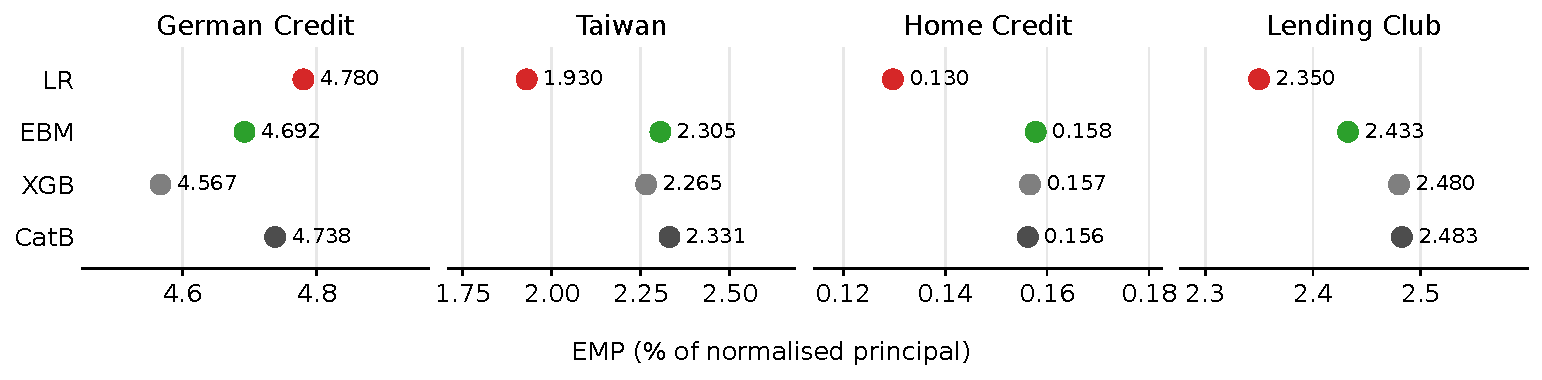
\includegraphics[width=\textwidth]{img/fig_emp_levels.pdf}
\caption[Economic performance by dataset and model]{Test-set EMP by dataset and model}
\label{fig:emp_levels}
\end{figure}

EMP among the three non-linear configurations spans $0.065$ percentage points on Taiwan
and $0.002$ on Home Credit. On Lending Club, XGBoost and CatBoost reach $2.480\%$ and
$2.483\%$, compared with $2.433\%$ for the EBM and $2.350\%$ for logistic regression, so
the ensemble--EBM differences are $0.047$ and $0.050$ percentage points of normalised
principal. German Credit shows a different point ordering, with logistic regression
reaching the highest EMP at $4.780\%$. 


\paragraph{Paired model comparisons.}
The point estimates establish the observed ordering, but not how sensitive the
between-model differences are to the composition of the held-out sample. The paired
bootstrap therefore evaluates whether the direction of the central cross-group
contrasts remains resolved under test-case resampling. Differences are defined as
$\Delta=a-b$, where $a$ is LR or the EBM and $b$ is XGBoost or CatBoost. An interval
entirely above zero indicates a higher numerical value for the intrinsically
interpretable model; one entirely below zero indicates a higher value for the
ensemble. An interval containing zero leaves the direction unresolved under this
procedure. Excluding zero does not establish practical relevance. The intervals are
unadjusted for multiplicity and conditional on the split, fitted pipelines and observed
class counts. Figure~\ref{fig:cross_group_differences} displays the four contrasts that
compare LR or the EBM directly with each boosted ensemble.

\begin{figure}[!htbp]
\centering
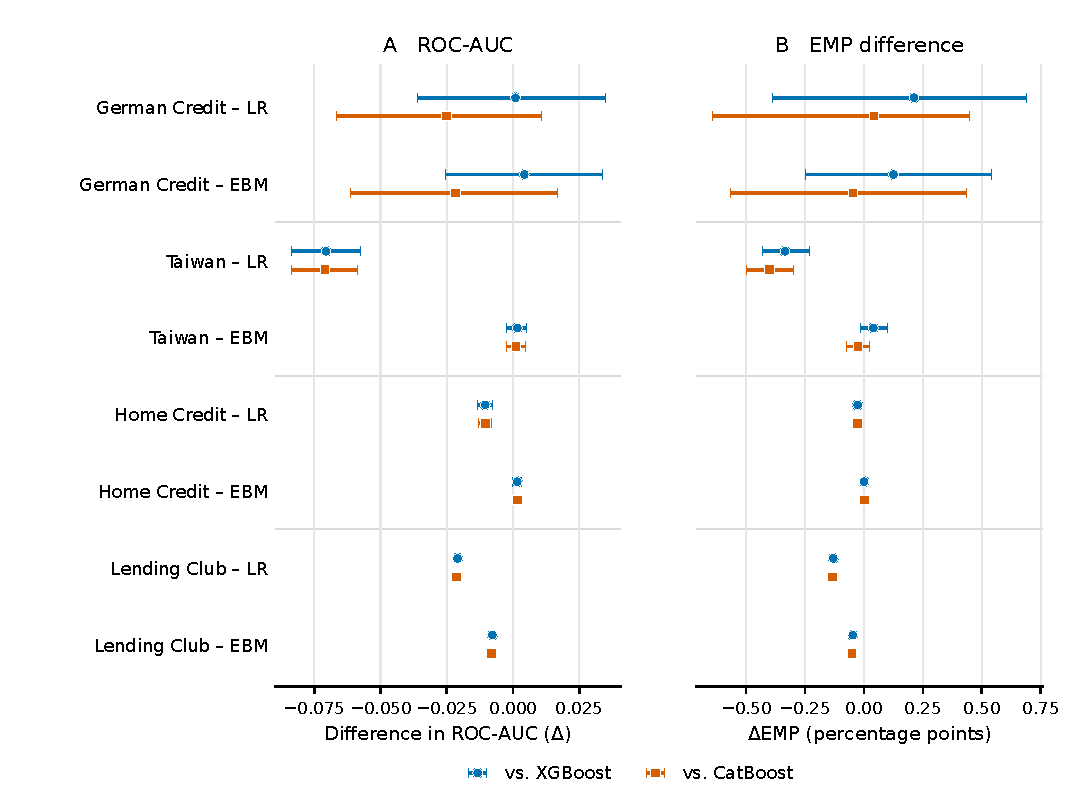
\includegraphics[width=0.90\textwidth]{img/fig_cross_group_differences.pdf}
\caption[Cross-group differences in ROC-AUC and EMP]{Cross-group differences in
ROC-AUC and EMP with unadjusted 95\% paired percentile-bootstrap intervals. Positive
values favour LR or the EBM; negative values favour the boosted ensemble.}
\label{fig:cross_group_differences}
\end{figure}

On German Credit, none of the EBM--ensemble intervals resolve a direction. On Taiwan,
all four EBM--ensemble intervals for ROC-AUC and EMP contain zero, so the procedure
resolves no direction there either. On Home Credit, the EBM is approximately level with
or slightly ahead of the ensembles: its ROC-AUC interval against CatBoost excludes zero,
whereas the interval against XGBoost narrowly contains it, and neither EMP interval
resolves a direction. In contrast, on Lending Club all four EBM--ensemble
intervals for ROC-AUC and EMP lie entirely below zero, so both ensembles lead the EBM on
both metrics. For logistic regression, the corresponding ROC-AUC and EMP intervals
against both ensembles also lie below zero on Taiwan and Lending Club.

The complete paired results for all six model pairs and all six metrics are reported in
Tables~\ref{tab:delta_pairs}, \ref{tab:delta_pairs_ap_brier} and
\ref{tab:delta_pairs_threshold}. German Credit produces the widest paired intervals,
consistent with its test partition of only $200$ observations; no paired interval for
any of the six metrics excludes zero there.

\section{Supplementary Evidence from Attribution Rankings}\label{sec:results-explainability}

The following analyses concern two properties of the global source-feature attribution
rankings: their stability under case resampling and their agreement across models. They
are not a comprehensive measurement of explainability or explanation quality.

\subsection{Case-Sampling Stability}\label{sec:results-stability}

For each pipeline, top-ten membership is the mean bootstrap inclusion frequency of the
ten features leading its original global ranking: a value of one means that these ten
features remain in the top ten in every resample. Rank-interval width is the mean width,
measured in rank positions, of their 95\% bootstrap rank intervals; smaller values
indicate less movement within the ranking.

Table~\ref{tab:shap_stability} reports these quantities conditional on the fitted
model--explainer pipelines. Mean top-ten membership ranges from $0.929$ to $1.000$, while
mean rank-interval width ranges from $0.20$ to $2.10$ positions.

The point estimates show no consistent stability advantage for logistic regression or
the EBM over XGBoost and CatBoost. This comparison is descriptive because no intervals
were computed for differences between pipelines; the reported rank intervals quantify
feature-rank variation within a pipeline, not uncertainty in between-pipeline
differences.

Absolute stability levels are not interpreted comparatively across datasets.
German Credit uses only $200$ explained test cases, whereas $2{,}000$ cases are
used for each larger dataset. In addition, the top ten account for $50.0\%$ of
the $20$ available source features on German Credit and $43.5\%$ of the $23$ on
Taiwan, compared with $13.9\%$ of the $72$ on Home Credit and $16.1\%$ of the
$62$ on Lending Club. Top-ten membership is therefore a less selective criterion
in the lower-dimensional datasets, additionally restricting direct comparison of
absolute stability levels.

\begin{table}[htbp]
\centering
\small
\begin{tabular}{llcc}
\toprule
\textbf{Dataset} & \textbf{Model} & \textbf{Top-10 membership}~$\uparrow$ & \textbf{Rank-interval width}~$\downarrow$ \\
\midrule
German Credit & LR & 1.000 & 2.00 \\
 & EBM & 0.929 & 2.10 \\
 & XGB & 1.000 & 1.40 \\
 & CatB & 0.998 & 1.40 \\
\midrule
Taiwan & LR & 0.988 & 0.90 \\
 & EBM & 1.000 & 0.80 \\
 & XGB & 1.000 & 0.20 \\
 & CatB & 0.980 & 1.10 \\
\midrule
Home Credit & LR & 1.000 & 0.40 \\
 & EBM & 0.997 & 0.70 \\
 & XGB & 0.965 & 0.80 \\
 & CatB & 0.964 & 0.40 \\
\midrule
Lending Club & LR & 0.989 & 0.70 \\
 & EBM & 1.000 & 0.60 \\
 & XGB & 0.998 & 0.60 \\
 & CatB & 0.999 & 0.40 \\
\bottomrule
\end{tabular}
\caption[Global attribution-rank stability under case resampling]{Case-sampling
stability of the ten features leading each original global ranking over $1{,}000$
bootstrap resamples.}
\label{tab:shap_stability}
\end{table}

\FloatBarrier

\subsection{Cross-Model Agreement}

Table~\ref{tab:cross_model_agreement} reports two complementary forms of agreement.
Jaccard is the size of the intersection of two top-ten sets divided by the size of their
union, so it ranges from zero for no shared feature to one for identical sets and is not
the share of features on which two pipelines agree. Mean pairwise Jaccard provides a
compact descriptive summary of top-ten overlap across the six model pairs. Spearman
correlation instead compares the ordering of the complete source-feature rankings and is
reported as a descriptive point estimate without an interval.

\begin{table}[htbp]
\centering
\fontsize{8.5pt}{10pt}\selectfont
\setlength{\tabcolsep}{3pt}
\begin{tabular}{@{}lccccccc@{}}
\toprule
 & \textbf{Jaccard [95\% bootstrap int.]} & \multicolumn{6}{c}{\textbf{Pairwise Spearman}~$\uparrow$} \\
\cmidrule(lr){2-2}\cmidrule(lr){3-8}
\textbf{Dataset} & \textbf{Mean pairwise} & \shortstack{LR\\EBM} & \shortstack{LR\\XGB} & \shortstack{LR\\CatB} & \shortstack{EBM\\XGB} & \shortstack{EBM\\CatB} & \shortstack{XGB\\CatB} \\
\midrule
German Credit & 0.717 [0.717, 0.747] & 0.89 & 0.82 & 0.88 & 0.89 & 0.91 & 0.95 \\
Taiwan        & 0.532 [0.486, 0.532] & 0.27 & 0.19 & 0.17 & 0.94 & 0.87 & 0.94 \\
Home Credit   & 0.649 [0.649, 0.696] & 0.92 & 0.88 & 0.89 & 0.97 & 0.97 & 0.99 \\
Lending Club  & 0.696 [0.696, 0.696] & 0.87 & 0.81 & 0.86 & 0.89 & 0.95 & 0.92 \\
\bottomrule
\end{tabular}
\caption[Cross-model agreement on which features matter]{Agreement between
model--explainer pipelines: mean pairwise top-ten Jaccard with its 95\% bootstrap
interval and pairwise Spearman correlations of the complete rankings.}
\label{tab:cross_model_agreement}
\end{table}

Mean pairwise top-ten Jaccard ranges from $0.532$ on Taiwan to $0.717$ on German Credit.
These raw levels are not read as a cross-dataset ordering, because the overlap expected
by chance increases as the number of available source features decreases. The degenerate
Lending Club interval reflects an unchanged mean overlap at the reported precision across
the central resamples. It does not imply an absence of uncertainty under retraining or
population change.

Agreement in the complete rankings is strongest among the three non-linear
configurations. Across datasets, the EBM's Spearman correlations with XGBoost and
CatBoost range from $0.87$ to $0.97$. Logistic regression remains broadly aligned on
German Credit, Home Credit and Lending Club but diverges on Taiwan, where its
correlations with the other models range from $0.17$ to $0.27$.

Table~\ref{tab:top_features} locates that divergence. All four Taiwan pipelines rank
\texttt{PAY\_0} first, but logistic regression fills the remaining top-five positions
with three bill-amount columns and \texttt{MARRIAGE}, whereas the three non-linear
configurations share \texttt{LIMIT\_BAL} and further repayment-status terms. The
divergence is therefore concentrated below the leading feature rather than spread
across the ranking.

\section{Sensitivity Analyses}

\subsection{Training-Set Size Sensitivity}\label{sec:size}

Figure~\ref{fig:learning_curves} reports test ROC-AUC and across-refit top-ten Jaccard
at the realised training sizes on Home Credit and Lending Club. Each value is the mean
of three refits under one manually specified configuration frozen across all sample sizes, each
refit drawing its own stratified subsample of that size from the training partition;
only the displayed grid points were run, so no behaviour between them is estimated.

\begin{figure}[htbp]
\centering
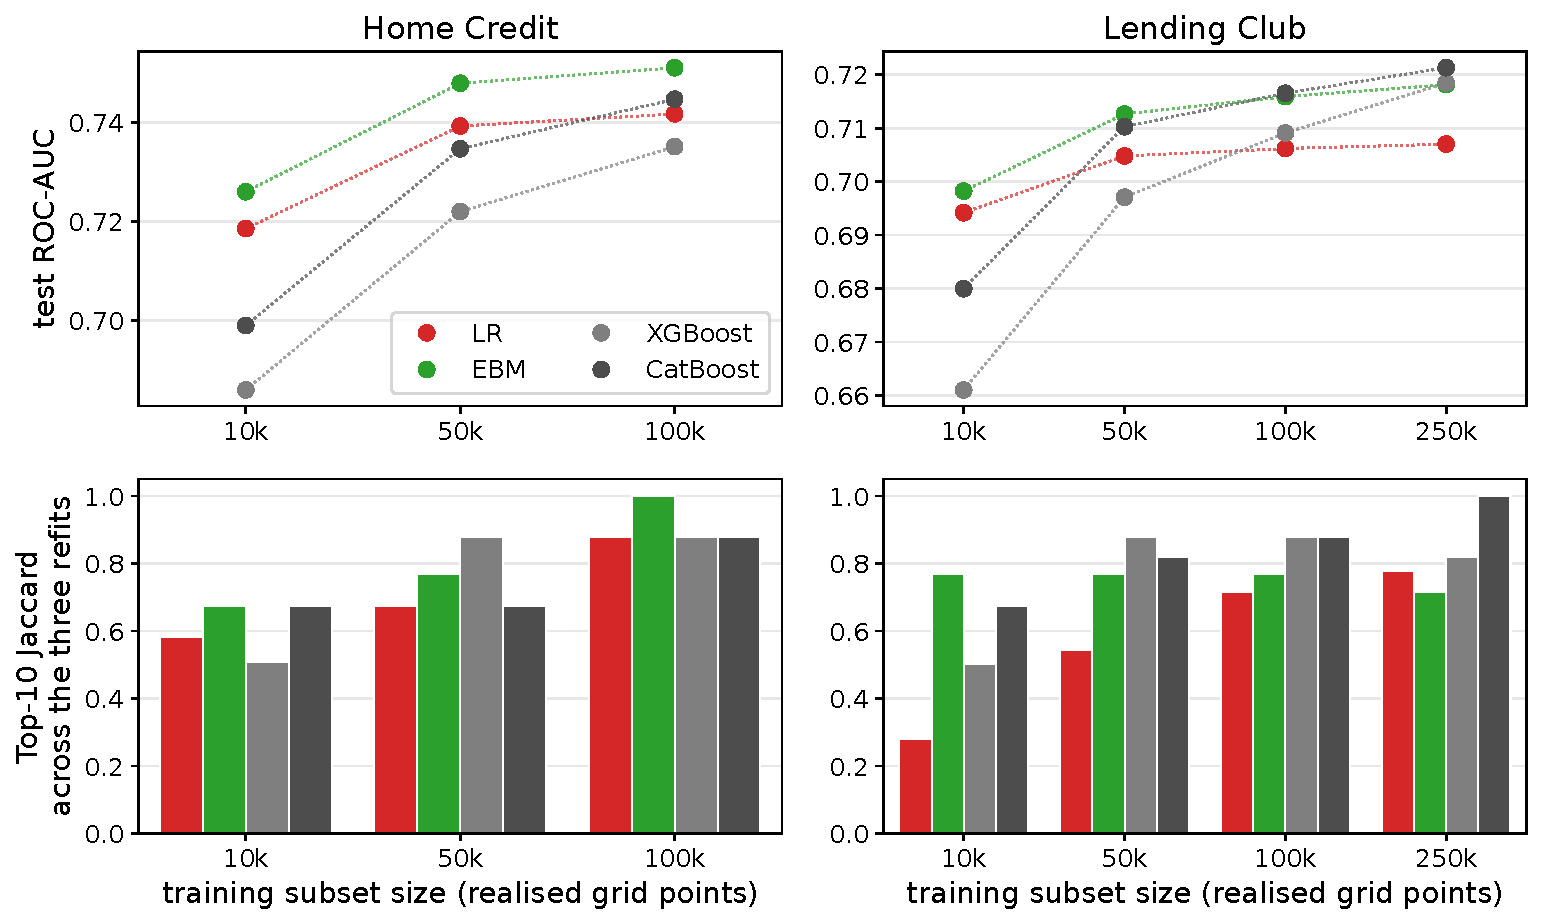
\includegraphics[width=\textwidth]{img/fig_learning_curves.pdf}
\caption[Training-size sensitivity of ROC-AUC and attribution-rank overlap]{Mean test
ROC-AUC (top) and mean pairwise top-ten Jaccard (bottom) across three refits at each
realised training size under fixed configurations.}
\label{fig:learning_curves}
\end{figure}

ROC-AUC rises across the realised grid for all four frozen configurations. XGBoost and
CatBoost show the largest numerical endpoint gains on both datasets, between $+0.041$
and $+0.057$, logistic regression the smallest, $+0.013$ and $+0.023$, and the EBM lies
between them. The maximum-minus-minimum ROC-AUC spread across the four configurations
narrows from $0.040$ to $0.016$ on Home Credit and from $0.037$ to $0.014$ on Lending
Club. The EBM remains above logistic regression at every realised size, while the two
ensembles close their initial deficits and have slightly higher endpoint estimates
on Lending Club.

These changes across the realised grid describe the training-size sensitivity of the
frozen configurations, not the general sample efficiency of optimally tuned model
families. The configurations differ
in capacity, only three repetitions were run per point, no interval was computed for
differences in change, and neither grid reaches the full headline training partition.
Across-refit top-ten Jaccard generally increases with training size, although not
monotonically for every configuration. On Home Credit, the endpoint values range from
approximately $0.88$ to $1.00$ at $100{,}000$ observations, compared with $0.50$ to
$0.67$ at $10{,}000$. On Lending Club, logistic regression rises from approximately
$0.28$ to $0.78$ and CatBoost from $0.67$ to $1.00$, whereas the EBM ends slightly below
its earlier values and XGBoost declines after reaching about $0.88$ at the intermediate
grid points.


\FloatBarrier

\subsection{Out-of-Time Evaluation}\label{sec:temporal-results}

\providecommand{\dbunit}{\setlength{\unitlength}{1mm}}
\providecommand{\dumbbell}[3]{%
  \raisebox{-0.4ex}{%
    \begingroup\dbunit
    \begin{picture}(42,2)(0,0)
      \linethickness{0.7mm}\put(#1,1){\line(1,0){#3}}
      \put(#1,1){\circle*{2}}
      \linethickness{0.25mm}\put(#2,1){\circle{2}}
    \end{picture}%
    \endgroup
  }%
}
\providecommand{\dbaxis}{%
  \raisebox{-0.4ex}{%
    \begingroup\dbunit
    \begin{picture}(42,5)(0,0)
      \linethickness{0.15mm}\put(0,5){\line(1,0){42}}
      \multiput(6.3,3.8)(10.5,0){4}{\line(0,1){1.2}}
      \put(6.3,0){\makebox(0,0)[b]{\scriptsize 0.70}}
      \put(16.8,0){\makebox(0,0)[b]{\scriptsize 0.71}}
      \put(27.3,0){\makebox(0,0)[b]{\scriptsize 0.72}}
      \put(37.8,0){\makebox(0,0)[b]{\scriptsize 0.73}}
    \end{picture}%
    \endgroup
  }%
}

Lending Club is the only dataset with an origination timestamp. The out-of-time run fits
on loans issued through 2014, tunes on 2015, refits through 2015 and evaluates the
resolved 2016--2018 cohort. Table~\ref{tab:oot_perf} compares it with the random-split
headline estimates.

\begin{table}[htbp]
\centering
\small
\begin{tabular}{@{}lccc@{}}
\toprule
\textbf{Model} & \textbf{ROC-AUC}~{\footnotesize($\bullet$~OOT, $\circ$~random)} & \shortstack{$\boldsymbol{\Delta}$~\textbf{ROC-AUC}\\{\footnotesize(OOT$-$random)}} & \shortstack{\textbf{EMP}\\{\footnotesize(\% of principal)}} \\
\midrule
LR       & \dumbbell{4.79}{14.19}{8.40}  & $-0.009$ & 1.97 \\
EBM      & \dumbbell{17.41}{27.99}{9.58} & $-0.010$ & 2.04 \\
XGBoost  & \dumbbell{22.23}{36.15}{12.92} & $-0.013$ & \textbf{2.06} \\
CatBoost & \dumbbell{22.40}{36.53}{13.13} & $-0.013$ & \textbf{2.06} \\
 & \dbaxis & & \\
\bottomrule
\end{tabular}
\caption[Lending Club out-of-time evaluation]{Random-split and out-of-time performance
on Lending Club, read off a common horizontal scale: the filled and hollow points denote
the out-of-time and random-split ROC-AUC, respectively, and their connecting segment
represents the descriptive difference $\Delta=\text{OOT}-\text{random}$. EMP is that of
the temporal run, under its own frozen economic configuration.}
\label{tab:oot_perf}
\end{table}

The out-of-time ROC-AUC estimates are between $0.009$ and $0.013$ below the corresponding
random-split estimates, while the broad point ordering---the two ensembles ahead of the
EBM and the EBM ahead of logistic regression---is retained.

Because the two ROC-AUC estimates arise from different training windows and
evaluation populations, $\Delta$ is a descriptive contrast between validation
designs rather than a paired estimate of temporal degradation.

On unrounded values, the EBM trails XGBoost and CatBoost by $0.0046$ and $0.0048$
ROC-AUC, respectively---approximately $0.005$ in both comparisons, against approximately
$0.008$ under the random split. No interval was computed for either design contrast or
for this difference of differences, so the numerical narrowing is descriptive.

Within the temporal run, the broad economic ordering is also retained: XGBoost and
CatBoost reach an EMP of $2.06\%$ of normalised principal, compared with $2.04\%$ for the
EBM and $1.97\%$ for logistic regression. These levels are comparable only within the
temporal run, because its class prior and return parameter are re-derived from the
temporal training window. The analysis concerns resolved loans only. Because
resolution-based selection becomes substantially stronger in the later vintages, the
observed out-of-time differences cannot be attributed to temporal population change
alone.

\chapter{Discussion}\label{ch:discussion}


\section{Performance and Economic Trade-offs}

Across the four datasets evaluated here, the EBM shows no uniform performance
disadvantage relative to the boosted ensembles. On Taiwan its ROC-AUC is effectively
level with XGBoost and CatBoost, and all four paired EBM--ensemble intervals contain
zero.

The Home Credit result is of a different kind. Here the EBM--CatBoost difference in
ROC-AUC lies entirely above zero, so on the second-largest test partition the only
EBM--ensemble contrast that resolves runs in favour of the glass-box model rather than
against it. It is the only such result in ROC-AUC, and it is narrow: the margin is
$0.0016$, the companion contrast against XGBoost includes zero at its lower bound, and
neither EMP interval resolves.

What it establishes is that a resolved direction in favour of the glass-box model
exists. Home Credit and Lending Club resolve in opposite directions, and the remaining
two resolve nothing. This supports the claim that an additive
model with a bounded number of fitted pairwise interactions can reach ensemble-level
discrimination in some tabular credit settings, consistent with prior reports
\citep{changHowInterpretableTrustworthy2021, dessainCostExplainabilityAI2023}. 

German Credit and Lending Club mark different limits to that conclusion. German Credit
provides too little test-sample precision to establish a stable statistical or economic
ordering: no paired interval for any metric excludes zero. Lending Club is the clear counterexample. XGBoost and CatBoost
lead the EBM by about $0.008$ ROC-AUC and by $0.047$--$0.050$ percentage points EMP,
with both EBM--ensemble contrasts resolved in ROC-AUC and in EMP under test-case
resampling.


EMP was included as a second evaluation dimension because ranking quality alone does not
capture the asymmetric consequences of credit decisions. On these datasets it largely
reproduces the statistical evaluation rather than adding an ordering of its own.

The EMP ordering matches the ROC-AUC ordering exactly on Home Credit and Lending
Club, these are the only two datasets in which an EBM--ensemble contrast resolves a direction. It
departs from that ordering only where the performance differences are unresolved to
begin with. Even where a direction does resolve, EMP acts as the more conservative
measure rather than an independent signal: on Home Credit the EBM--CatBoost contrast
excludes zero in ROC-AUC but not in EMP. Nowhere does the profit measure reverse a
direction that discrimination has already resolved.

Its contribution here is therefore not necessarily a second ordering but a second unit. A gap of
$0.008$ ROC-AUC cannot be weighed against anything on its own, but expressed in percentage
points of normalised principal, the same gap becomes a quantity an institution can hold
against the cost of the alternative.

Under the EMP parameterisation, the observed Lending Club difference can be read as a
modelled economic price. The EBM's EMP is $0.047$--$0.050$ percentage points of
normalised principal below that of the two ensembles. This corresponds to approximately
EUR~$0.50$ per EUR~$1{,}000$ of normalised principal, compared with an EMP level of
about EUR~$24.80$ per EUR~$1{,}000$. The difference therefore amounts to approximately
$2\%$ of the modelled EMP level.

Because EMP levels are not directly comparable across datasets, the interpretation
focuses on paired model differences within each dataset. Only Lending Club yields paired
EBM--ensemble EMP intervals that exclude zero. On Home Credit, the point estimates favour
the EBM, but both paired difference intervals include zero and neither contrast is resolved
on Taiwan. Profit-based
evaluation therefore identifies a modelled economic disadvantage for the EBM in only one
of four settings, while its direction remains unresolved in the other three.

Because all configurations are tuned to maximise validation ROC-AUC, this high agreement between the metrics is partly induced by the experimental design. The EMP figures therefore serve as an economic lens applied to standard, discrimination-optimised pipelines, quantifying the economic consequences of models chosen solely for their statistical ranking power.

Logistic regression serves an important comparative role by helping to distinguish
intrinsic interpretability from the restrictions of a linear functional form. Although
it attains the highest threshold-metric point estimates on the small German Credit
dataset, it is consistently less competitive with the non-linear models across the 
larger datasets. This pattern shows that direct inspectability alone is insufficient 
for model choice. An interpretable model must also provide sufficient functional 
flexibility for the empirical setting. The EBM therefore provides the more informative 
test of whether inherent interpretability can exist alongside competitive performance.

\section{Explanation Stability, Agreement and Interpretability}

Under case resampling, top-ten membership is high across all four pipelines and partly
compressed by the small feature vocabularies of German Credit and Taiwan. The more
discriminating rank-interval widths lead to the same substantive conclusion: neither LR
nor the EBM shows a consistent stability advantage over XGBoost and CatBoost.

Cross-model agreement provides a different form of evidence. Top-ten Jaccard indicates
partial overlap between the features prioritised by the pipelines, while the complete
rankings place the EBM close to the two ensembles; logistic regression diverges most
strongly on Taiwan. This agreement indicates similarity in global feature priorities,
but it does not identify a correct or faithful ranking, because attribution allocation
depends on the fitted model, explainer semantics and feature dependence
\citep{aasExplainingIndividualPredictions2021}.

For model choice, the explanation measures therefore add two qualifications. They
provide no stability-based reason to prefer the intrinsically interpretable pipelines,
but they show that the EBM and the ensembles often emphasise similar source features.
The relevant interpretability distinction remains structural: LR and the EBM expose
components of their fitted prediction functions, whereas XGBoost and CatBoost require a
separate post-hoc explanation computation
\citep{rudinStopExplainingBlack2019a}. The case for the EBM consequently rests on this
direct inspectability together with its observed performance, not on superior measured
attribution stability.


\section{Sensitivity to Training Size and Time}

The learning curves show that relative model performance changes with training-set
size under the fixed configurations examined. XGBoost and CatBoost gain more
ROC-AUC as the sample grows. The EBM remains ahead of logistic regression, while
the ensembles close or reverse their initial deficits. The EBM is therefore more
competitive at smaller sample sizes in these experiments, whereas the boosted-tree
ensembles benefit more from additional data. Across-refit top-ten Jaccard overlap
does not increase monotonically, indicating that larger training samples do not
consistently produce more reproducible global feature rankings.

The out-of-time evaluation yields lower ROC-AUC estimates for all Lending Club
pipelines but preserves their random-split ordering: XGBoost and CatBoost lead,
followed by the EBM and logistic regression. The same point-estimate hierarchy
appears for EMP. The chronological evaluation therefore reproduces the central
Lending Club pattern in both discrimination and economic performance. The
EBM--ensemble ROC-AUC gap is nevertheless narrower than under the random split:
the direction of the observed difference recurs, while its magnitude changes.
Taken together, these analyses show that key elements of the model ordering remain across alternative settings: the EBM remains ahead of logistic regression across
the evaluated training sizes, and the Lending Club random-split ordering is
reproduced under temporal evaluation.


\section{Relation to Prior Findings}

\citet{bahloolPerformanceFairnessExplainability2026} characterise the
performance--explainability trade-off in credit scoring as more often assumed than
empirically quantified, because performance and explainability are commonly studied
separately. The present findings support that diagnosis. An ensemble advantage over the EBM resolves only on Lending Club, whereas
one ROC-AUC comparison on Home Credit resolves in the opposite direction and the
remaining comparisons show no consistent ensemble advantage. This establishes no equivalence. It does shift the burden of argument: a claim that
intrinsic interpretability entails a predictive cost requires evidence in the setting
where it is made and comparison with functionally flexible glass-box alternatives
rather than linear baselines alone.

The observed magnitudes are broadly consistent with the closest quantitative reference
points. Across 45 tabular datasets,
\citet{amekoeExploringAccuracyInterpretability2024b} report an average relative
accuracy loss below $4\%$ for intelligible models.
\citet{dessainCostExplainabilityAI2023} report fifteen to twenty basis points of
return between their best black-box and interpretable models, against about five
basis points of normalised principal here. These quantities are not directly
comparable. The first measures accuracy across a wider tabular benchmark, while
the second measures realised return rather than EMP. They nevertheless support the
same broader interpretation: where a performance cost exists, its magnitude must be
evaluated in context rather than inferred from the model family alone.

The Lending Club results contextualise the findings of \citet{schwartzEnhancingMLModels2025}, 
who report the EBM narrowly outperforming an XGBoost baseline on the same raw dataset 
(ROC-AUC $0.674$ versus $0.669$). The present study instead yields a consistent but small 
ensemble advantage in both ROC-AUC and economic value. This contrast does not necessarily 
indicate contradictory model behaviour. Rather, it highlights how sensitive relative 
performance is to specific pipeline configurations and empirical contexts. Whether the 
EBM slightly leads or slightly trails the tree ensembles ultimately depends on design 
choices such as feature selection and evaluation criteria. The shared conclusion across 
both pipelines, however, is that the EBM performs at a highly competitive level. It 
therefore emerges not as a mere transparency-oriented fallback, but as a primary model 
candidate whose exact rank must be established in the target context.

\section{Regulatory Context}\label{sec:regulatory-reading}

The framework set out in Section~\ref{sec:regulatory} does not translate the
applicable legal requirements into a preference for a particular model family.
Neither the AI Act nor the GDPR makes an EBM compliant by construction or a
boosted ensemble non-compliant because its explanations are generated post hoc.
The legal assessment instead concerns the deployed system, including its intended
use, documentation, data governance, human oversight, monitoring and the
information provided to affected persons. Model architecture may supply relevant
technical evidence but cannot replace this system-level assessment.

The evaluated model families nevertheless differ structurally in how explanation
evidence is generated. Logistic regression and the EBM expose components of their
fitted prediction functions, whereas XGBoost and CatBoost require a separate
TreeSHAP computation. As \citet{liptonMythosModelInterpretability2018} stresses,
a post-hoc explanation is not equivalent to direct transparency of the fitted
model. This distinction affects how model behaviour can be documented and
examined, but it alone establishes neither legal sufficiency nor a ranking of
compliance effort. Direct inspectability does not prove compliance, while reliance
on TreeSHAP does not prove non-compliance.

The empirical metrics reported in this thesis may inform the assessment of a
deployed system, but none constitutes a statutory threshold or conformity finding.
Accordingly, neither architecture is excluded on model-family grounds, and this
thesis does not assess whether any evaluated pipeline satisfies the applicable
requirements.

\section{Implications for Model Choice}

The central implication is procedural: model selection should not begin from a
presumed performance penalty for intrinsic interpretability. While 
\citet{amekoeExploringAccuracyInterpretability2024b} recommend incorporating inherently 
interpretable models primarily when transparency is a key constraint, the marginality of 
the trade-offs demonstrated in this thesis suggests that the EBM should enter the 
initial candidate set alongside boosted-tree ensembles from the outset. Rather than 
serving as a transparency-oriented fallback after a black-box model has already 
been selected, the glass-box model must be evaluated on its own predictive and 
economic merits. Its direct inspectability is an additional structural property, 
not its sole justification.


\section{Limitations}\label{sec:limitations}

Several design choices constrain the generalisability of the findings and define
the limits of the evaluated empirical setup.

\paragraph{Data and population.}
All four datasets contain only \emph{booked} loans. The findings are therefore
conditional on historical acceptance decisions and do not evaluate model performance
for the through-the-door applicant population. No reject-inference procedure was
applied. Moreover, the datasets are historical public benchmarks and represent
contemporary operational credit scoring only partially. Changes in lending products,
underwriting policies, macroeconomic conditions, applicant behaviour and the
availability of decision-time information may alter both predictive relationships and
relative model performance. The findings should therefore be interpreted as evidence
under the evaluated benchmark conditions rather than as expected performance for a
current institution-specific applicant population. No group-wise fairness evaluation was conducted, so the results support no conclusions
about disparate outcomes across applicant groups.

\paragraph{Model coverage.}
Each side of the comparison rests on limited model families. The flexible side is
represented by gradient-boosted trees in two implementations, chosen because they are
the documented reference for tabular credit data, but neural architectures, random
forests and other flexible learners were not evaluated. The intrinsically interpretable
side is represented by one non-linear model, so the within-family check available for
the ensembles has no counterpart there. Findings on the EBM consequently may not transfer
to other interpretable classes and
the conclusions concern the four evaluated pipelines rather than the model classes as a
whole.

\paragraph{Feature representation.}
Feature encoding is not neutral between model families. Ordinal encodings represent
ordered variables in a form that the models may use differently, while aggregating
one-hot encoded columns into source-feature importances can affect the resulting
attribution rankings. These effects were not isolated experimentally. The reported
comparisons therefore partly reflect interactions between the algorithms and the
chosen feature representation rather than model-class differences alone.

\paragraph{Model selection and tuning.}
All configurations were selected to maximise validation ROC-AUC. The EMP results
therefore describe the economic performance of pipelines selected for their overall
discriminatory ability rather than pipelines optimised directly for expected profit.
These objectives need not select the same configuration: ROC-AUC evaluates ranking
across the full range of decision thresholds, whereas EMP rewards ranking performance
in the regions that are economically relevant under its assumed returns, losses and
class prevalence. A configuration with a slightly lower ROC-AUC could consequently
produce a higher EMP. Direct EMP-based tuning might therefore change
both the selected configurations and the relative ordering of the model families. The
profit-based comparison is conditional on the discrimination-first selection strategy
and does not establish which models would perform best under direct economic
optimisation.

\paragraph{Uncertainty and temporal coverage.}
The headline results rest on one train--test split per dataset. The paired bootstrap
quantifies test-set sampling uncertainty conditional on the fitted pipelines. It does
not propagate uncertainty from alternative splits, repeated model selection or
alternative explainer reference samples. No uncertainty intervals were calculated for
between-pipeline differences in attribution-ranking stability, so their relative
ordering remains descriptive.

Out-of-time evaluation was possible only for Lending Club and uses a single
chronological design rather than repeated rolling-origin assessments. It is also
subject to maturity-dependent censoring because later cohorts contain a smaller
proportion of loans with resolved outcomes. The temporal analysis therefore cannot
separate changes caused via temporal drift from those caused by changing outcome
availability, nor does it establish that the observed ordering persists across
successive origination cohorts or under changing market conditions.

\paragraph{Metrics and explanations.}
EMP remains conditional on the assumed return, loss-given-default distribution and
class prevalence. The use of a common loss distribution and partly standardised return
assumptions enables a consistent experimental comparison across the datasets, but it
does not reproduce the specific economics of each credit product or lending
institution. Product-specific estimates of returns and loss severity could shift the
economically relevant operating region and thereby change not only absolute EMP levels,
but also the pairwise differences and potentially the model ordering. The reported EMP
results therefore describe economic performance under the stated assumptions rather
than realised portfolio profit or a definitive profitability ranking
\citep{xuProfitRiskdrivenCredit2024}.

The explanation analysis combines model-specific methods with different reference
constructions and decomposition rules. Its results consequently describe
model--explainer pipelines rather than model properties alone. Attribution-ranking
stability measures the reproducibility of global rankings under case resampling. It
does not test whether those rankings faithfully represent the features governing the
fitted model's predictions. Human intelligibility and the usefulness of local
explanations to credit decision-makers or applicants were likewise not evaluated.

\paragraph{Evidence base.}
The closest prior comparison, \citet{schwartzEnhancingMLModels2025}, is a preprint. It
was retained because it is the only identified study evaluating the EBM against
XGBoost on Lending Club, and omitting the closest precedent would have left the
comparison without a direct reference point. Its reported values should nevertheless be
treated as unverified. Two circumstances limit the resulting reliance. First, the
preprint enters the discussion as a contrast rather than as support: it reports the EBM
narrowly ahead of XGBoost, whereas the present study finds a small ensemble advantage on
the same dataset. Second, the broader interpretation that flexible interpretable models
can be competitive is carried by peer-reviewed evidence
\citep{amekoeExploringAccuracyInterpretability2024b}.


\section{Future Work}\label{sec:future}

A deployment-oriented extension should evaluate the pipelines on current institutional
credit data collected at a consistent decision point. Reject-inference and sensitivity
analyses could examine whether the relative model performance extends beyond the booked
population, while prespecified group-fairness
analyses could test whether the observed performance differences persist across
relevant applicant groups. Product-specific
estimates of returns, loss severity and class prevalence would additionally indicate
whether the economic ordering obtained under the standardised EMP assumptions transfers
to operational portfolios.

Repeating the full pipeline across independently drawn data partitions would propagate
sources of uncertainty held fixed in the present design and permit direct estimation of
between-pipeline differences in attribution-ranking stability.

EMP-based or
multi-objective hyperparameter selection could test whether discrimination-first tuning
conceals configurations with preferable economic trade-offs. Temporal validation also
warrants extension to additional datasets with reliable origination timestamps and
sufficiently mature outcomes.

Extending the model set would test how broadly the observed performance pattern applies.
Additional glass-box approaches could show whether the EBM's competitiveness is specific
to its architecture or extends to other intrinsically interpretable models. Including
flexible predictors beyond boosted trees would likewise test whether the findings hold
against a larger set of black-box alternatives.

Explanation evaluation should distinguish stability from faithfulness and practical
usefulness. Retraining- or perturbation-based tests designed to limit unrealistic
out-of-distribution inputs could assess whether the attributed features accurately
represent the fitted model's predictive behaviour
\citep{zhengFFidelityRobustFramework2025}. Local explanations could then be evaluated
with credit decision-makers and affected applicants to determine whether they are
understandable, decision-relevant and useful for understanding or contesting individual
outcomes \citep{nautaAnecdotalEvidenceQuantitative2023}.

Finally, a controlled organisational study could examine whether direct inspectability
changes the resources required to document, validate, maintain and communicate a
credit-scoring system relative to a separate post-hoc explanation pipeline. Relevant
outcomes include development and validation time, documentation obligations,
explainer-specific failure modes and stakeholder comprehension. The structural and
regulatory differences between inherent and post-hoc explanations motivate this
comparison but do not predetermine its result.


\chapter{Conclusion}\label{ch:conclusion}

This thesis examined how intrinsically interpretable credit-scoring models, particularly the Explainable Boosting Machine (EBM), compare with post-hoc-explained boosted-tree ensembles in predictive and profit-based performance and what the observed differences imply for model choice in the EU regulatory context. Under the empirical conditions studied, choosing the EBM did not entail a consistent performance penalty relative to XGBoost and CatBoost. A predictive and economic ensemble advantage emerged on Lending Club, but this pattern did not recur across the other datasets. The findings establish neither model-class equivalence nor a universally preferable architecture. They instead support including functionally flexible glass-box models in the initial empirical model-selection process rather than treating them solely as transparency-oriented alternatives. In the EU regulatory context, neither architecture is compliant or non-compliant by construction; conformity must be assessed for the complete deployed system.

The contrast between logistic regression and the EBM shows why the performance of a transparent linear baseline cannot be generalised to intrinsically interpretable models as a broader class. By combining direct inspectability with greater functional flexibility, the EBM remained more competitive with the boosted ensembles than logistic regression. Expected Maximum Profit largely reinforced the ordering indicated by discrimination while expressing the observed differences in economic terms under the stated assumptions. The explanation analysis found no consistent case-sampling stability advantage for the intrinsically interpretable pipelines. Although the EBM and the ensembles frequently prioritised similar source features, the analysis did not test whether these rankings accurately represented the models' predictive behaviour or were useful to credit decision-makers or affected applicants. The observed performance gaps also changed with training-set size, while the Lending Club ordering recurred under chronological evaluation. Within these sensitivity analyses, the precise performance gaps varied more than the model ordering.

These conclusions remain bounded by historical public datasets containing only booked loans, without reject inference or group-fairness evaluation. The principal comparisons rely on one train--test partition per dataset and a single temporal design, while EMP remains conditional on assumed economic parameters and ROC-AUC-based model selection. Moreover, the explanation analysis is restricted to the reproducibility and similarity of global feature rankings. These limitations restrict direct generalisation to contemporary institutional credit-scoring systems.

Future research should therefore evaluate these pipelines on current institutional data covering broader applicant populations, using product-specific economic assumptions and explicit fairness analyses. Repeated end-to-end model selection, EMP-based or multi-objective tuning and rolling-origin validation could determine whether the observed performance patterns persist when selection and temporal uncertainty are propagated more fully. Additional tests should examine whether the resulting explanations accurately represent model behaviour, whether they are understandable and useful to their intended audiences, and whether they can support the provision of intelligible individual explanations where legally required. Controlled organisational studies could further investigate whether direct inspectability reduces the effort required to document, validate and communicate a credit-scoring system under the applicable regulatory requirements.




% Bibliography
% Bibliography
% Bibliography
\cleardoublepage
\addcontentsline{toc}{chapter}{Bibliography}

\nocite{EUAIAct2024}

\bibliographystyle{apacite}
\bibliography{bibliography}

% Appendix (if required...)
\appendix

\chapter{Implementation Details}\label{app:repro_details}

\section{Search Space and Selected Hyperparameters}\label{app:hyperparams}

Table~\ref{tab:hp_all} gives the prespecified search space and, beside it, the
configuration selected once per model and dataset, which is the configuration that was refitted,
calibrated, evaluated and explained. Settings not listed use the library defaults. The
search space is identical across datasets. The logistic-regression grid is enumerated
exhaustively at its $6$ points; the remaining spaces are sampled by randomized search at
budgets of $20$, $30$ and $20$ evaluations, and the EBM's \texttt{outer\_bags} is fixed
at $8$.

\begin{table}[htbp]
\centering
\footnotesize
\setlength{\tabcolsep}{3.5pt}
\begin{tabular}{@{}ll>{\raggedright\arraybackslash}p{3.0cm}cccc@{}}
\toprule
                 &                         &                        & \multicolumn{4}{c}{\textbf{Selected}}                                                  \\
\cmidrule(lr){4-7}
\textbf{Model}   & \textbf{Hyperparameter} & \textbf{Search values} & \shortstack{German\\Credit} & Taiwan & \shortstack{Home\\Credit} & \shortstack{Lending\\Club} \\
\midrule
LR               & $C$                     & 0.001, 0.01, 0.1, 1, 10, 100 & 0.01  & 100   & 10    & 10      \\
\midrule
EBM              & interactions            & 10, 20                       & 20    & 10    & 20    & 20      \\
                 & max\_leaves             & 2, 3, 5                      & 2     & 3     & 2     & 2       \\
                 & max\_bins               & 256, 512                     & 256   & 512   & 256   & 512     \\
                 & learning rate           & 0.005, 0.01, 0.02, 0.05      & 0.01  & 0.05  & 0.01  & 0.05    \\
                 & min\_samples\_leaf      & 2, 5                         & 5     & 5     & 5     & 2       \\
\midrule
XGBoost          & max\_depth              & 4, 6, 8                      & 4     & 6     & 4     & 6       \\
                 & learning rate           & 0.03, 0.05, 0.1              & 0.03  & 0.05  & 0.03  & 0.03    \\
                 & subsample               & 0.8, 1.0                     & 0.8   & 0.8   & 0.8   & 0.8     \\
                 & colsample\_bytree       & 0.8, 1.0                     & 1.0   & 0.8   & 1.0   & 1.0     \\
                 & min\_child\_weight      & 1, 5                         & 5     & 5     & 5     & 1       \\
                 & gamma                   & 0, 0.1                       & 0     & 0     & 0.1   & 0       \\
                 & n\_estimators           & early stopping               & 92    & 78    & 895   & 1{,}762 \\
\midrule
CatBoost         & depth                   & 4, 6, 8                      & 8     & 6     & 4     & 6       \\
                 & learning rate           & 0.03, 0.05, 0.1              & 0.1   & 0.05  & 0.05  & 0.1     \\
                 & l2\_leaf\_reg           & 1, 3, 5                      & 3     & 5     & 3     & 5       \\
                 & iterations              & early stopping               & 37    & 192   & 941   & 1{,}530 \\
\bottomrule
\end{tabular}
\caption[Search space and selected hyperparameters]{Search space and selected
  hyperparameters.}
\label{tab:hp_all}
\end{table}

\FloatBarrier

\chapter{Supplementary Results}\label{app:supplementary}

\section{Performance and Bootstrap Details}

\begingroup
\makeatletter
\setlength{\@fptop}{0pt}
\makeatother

\begin{table}[!t]
\centering
\footnotesize
\setlength{\tabcolsep}{4pt}
\begin{tabular}{@{}llrcrc@{}}
\toprule
                 &                     & \multicolumn{2}{c}{$\Delta$ROC-AUC} & \multicolumn{2}{c}{\shortstack{$\Delta$EMP\\(percentage points)}} \\
\cmidrule(lr){3-4}\cmidrule(lr){5-6}
\textbf{Dataset} & \textbf{Pair}~$a-b$ & \textbf{Point} & \shortstack{\textbf{95\% bootstrap}\\\textbf{interval}} & \textbf{Point} & \shortstack{\textbf{95\% bootstrap}\\\textbf{interval}} \\
\midrule
German Credit    & LR $-$ EBM   & $-0.0033$ & $[-0.0368,\ +0.0270]$   & $+0.088$  & $[-0.495,\ +0.464]$ \\
                 & LR $-$ XGB   & $+0.0010$ & $[-0.0362,\ +0.0348]$   & $+0.212$  & $[-0.387,\ +0.690]$ \\
                 & LR $-$ CatB  & $-0.0251$ & $[-0.0664,\ +0.0107]$   & $+0.042$  & $[-0.643,\ +0.448]$ \\
                 & EBM $-$ XGB  & $+0.0043$ & $[-0.0256,\ +0.0337]$   & $+0.125$  & $[-0.248,\ +0.543]$ \\
                 & EBM $-$ CatB & $-0.0218$ & $[-0.0614,\ +0.0169]$   & $-0.046$  & $[-0.569,\ +0.434]$ \\
                 & XGB $-$ CatB & $-0.0261$ & $[-0.0576,\ +0.0058]$   & $-0.171$  & $[-0.703,\ +0.293]$ \\
\midrule
Taiwan           & LR $-$ EBM   & $-0.0722$ & $[-0.0846,\ -0.0589]$   & $-0.376$  & $[-0.474,\ -0.271]$ \\
                 & LR $-$ XGB   & $-0.0705$ & $[-0.0835,\ -0.0576]$   & $-0.336$  & $[-0.433,\ -0.231]$ \\
                 & LR $-$ CatB  & $-0.0710$ & $[-0.0838,\ -0.0587]$   & $-0.401$  & $[-0.500,\ -0.298]$ \\
                 & EBM $-$ XGB  & $+0.0016$ & $[-0.0024,\ +0.0052]$   & $+0.040$  & $[-0.014,\ +0.099]$ \\
                 & EBM $-$ CatB & $+0.0012$ & $[-0.0024,\ +0.0049]$   & $-0.026$  & $[-0.075,\ +0.023]$ \\
                 & XGB $-$ CatB & $-0.0004$ & $[-0.0036,\ +0.0032]$   & $-0.065$  & $[-0.119,\ -0.017]$ \\
\midrule
Home Credit      & LR $-$ EBM   & $-0.0121$ & $[-0.0146,\ -0.0096]$   & $-0.028$  & $[-0.040,\ -0.017]$ \\
                 & LR $-$ XGB   & $-0.0105$ & $[-0.0132,\ -0.0079]$   & $-0.027$  & $[-0.042,\ -0.014]$ \\
                 & LR $-$ CatB  & $-0.0105$ & $[-0.0130,\ -0.0080]$   & $-0.026$  & $[-0.040,\ -0.013]$ \\
                 & EBM $-$ XGB  & $+0.0016$ & $[-0.000006,\ +0.0031]$ & $+0.001$  & $[-0.007,\ +0.010]$ \\
                 & EBM $-$ CatB & $+0.0016$ & $[+0.0003,\ +0.0030]$   & $+0.002$  & $[-0.006,\ +0.010]$ \\
                 & XGB $-$ CatB & $+0.0000$ & $[-0.0012,\ +0.0012]$   & $+0.0004$ & $[-0.007,\ +0.008]$ \\
\midrule
Lending Club     & LR $-$ EBM   & $-0.0131$ & $[-0.0141,\ -0.0122]$   & $-0.083$  & $[-0.091,\ -0.075]$ \\
                 & LR $-$ XGB   & $-0.0209$ & $[-0.0220,\ -0.0197]$   & $-0.130$  & $[-0.139,\ -0.120]$ \\
                 & LR $-$ CatB  & $-0.0213$ & $[-0.0224,\ -0.0201]$   & $-0.133$  & $[-0.142,\ -0.124]$ \\
                 & EBM $-$ XGB  & $-0.0078$ & $[-0.0085,\ -0.0069]$   & $-0.047$  & $[-0.054,\ -0.040]$ \\
                 & EBM $-$ CatB & $-0.0081$ & $[-0.0088,\ -0.0074]$   & $-0.050$  & $[-0.057,\ -0.043]$ \\
                 & XGB $-$ CatB & $-0.0004$ & $[-0.0008,\ +0.0001]$   & $-0.003$  & $[-0.008,\ +0.001]$ \\
\bottomrule
\end{tabular}
\caption[Paired differences in ROC-AUC and EMP]{Paired test-set differences
  ($\Delta=a-b$) with unadjusted 95\% percentile-bootstrap intervals; positive values
  denote a higher numerical value for model $a$. EMP differences are percentage points.}
\label{tab:delta_pairs}
\end{table}

\begin{table}[!t]
\centering
\fontsize{8.5pt}{10pt}\selectfont
\setlength{\tabcolsep}{2pt}
\begin{tabular}{@{}llrcrc@{}}
\toprule
                 &                     & \multicolumn{2}{c}{$\Delta$AP} & \multicolumn{2}{c}{$\Delta$Brier score} \\
\cmidrule(lr){3-4}\cmidrule(lr){5-6}
\textbf{Dataset} & \textbf{Pair}~$a-b$ & \textbf{Point} & \shortstack{\textbf{95\% bootstrap}\\\textbf{interval}} & \textbf{Point} & \shortstack{\textbf{95\% bootstrap}\\\textbf{interval}} \\
\midrule
German Credit    & LR $-$ EBM   & $+0.0508$ & $[-0.0261,\ +0.1206]$ & $-0.001121$ & $[-0.016059,\ +0.014775]$ \\
                 & LR $-$ XGB   & $+0.0148$ & $[-0.0489,\ +0.0718]$ & $-0.007013$ & $[-0.021542,\ +0.007840]$ \\
                 & LR $-$ CatB  & $-0.0392$ & $[-0.1197,\ +0.0359]$ & $+0.004357$ & $[-0.015050,\ +0.025222]$ \\
                 & EBM $-$ XGB  & $-0.0361$ & $[-0.1085,\ +0.0449]$ & $-0.005892$ & $[-0.018557,\ +0.006894]$ \\
                 & EBM $-$ CatB & $-0.0900$ & $[-0.1761,\ +0.0001]$ & $+0.005478$ & $[-0.012942,\ +0.023911]$ \\
                 & XGB $-$ CatB & $-0.0539$ & $[-0.1190,\ +0.0125]$ & $+0.011370$ & $[-0.003607,\ +0.026075]$ \\
\midrule
Taiwan           & LR $-$ EBM   & $-0.0576$ & $[-0.0743,\ -0.0384]$ & $+0.007031$ & $[+0.004854,\ +0.008976]$ \\
                 & LR $-$ XGB   & $-0.0628$ & $[-0.0789,\ -0.0455]$ & $+0.007475$ & $[+0.005495,\ +0.009332]$ \\
                 & LR $-$ CatB  & $-0.0618$ & $[-0.0768,\ -0.0452]$ & $+0.007465$ & $[+0.005665,\ +0.009194]$ \\
                 & EBM $-$ XGB  & $-0.0053$ & $[-0.0164,\ +0.0053]$ & $+0.000444$ & $[-0.000640,\ +0.001660]$ \\
                 & EBM $-$ CatB & $-0.0043$ & $[-0.0143,\ +0.0049]$ & $+0.000434$ & $[-0.000506,\ +0.001531]$ \\
                 & XGB $-$ CatB & $+0.0010$ & $[-0.0075,\ +0.0095]$ & $-0.000010$ & $[-0.000917,\ +0.000877]$ \\
\midrule
Home Credit      & LR $-$ EBM   & $-0.0157$ & $[-0.0202,\ -0.0113]$ & $+0.000771$ & $[+0.000596,\ +0.000939]$ \\
                 & LR $-$ XGB   & $-0.0141$ & $[-0.0193,\ -0.0087]$ & $+0.000715$ & $[+0.000510,\ +0.000906]$ \\
                 & LR $-$ CatB  & $-0.0140$ & $[-0.0183,\ -0.0090]$ & $+0.000670$ & $[+0.000493,\ +0.000836]$ \\
                 & EBM $-$ XGB  & $+0.0016$ & $[-0.0013,\ +0.0048]$ & $-0.000056$ & $[-0.000167,\ +0.000059]$ \\
                 & EBM $-$ CatB & $+0.0017$ & $[-0.0007,\ +0.0043]$ & $-0.000101$ & $[-0.000201,\ -0.000004]$ \\
                 & XGB $-$ CatB & $+0.0001$ & $[-0.0023,\ +0.0024]$ & $-0.000044$ & $[-0.000130,\ +0.000033]$ \\
\midrule
Lending Club     & LR $-$ EBM   & $-0.0164$ & $[-0.0182,\ -0.0147]$ & $+0.001962$ & $[+0.001815,\ +0.002114]$ \\
                 & LR $-$ XGB   & $-0.0265$ & $[-0.0284,\ -0.0245]$ & $+0.003212$ & $[+0.003022,\ +0.003384]$ \\
                 & LR $-$ CatB  & $-0.0273$ & $[-0.0291,\ -0.0253]$ & $+0.003306$ & $[+0.003122,\ +0.003478]$ \\
                 & EBM $-$ XGB  & $-0.0101$ & $[-0.0115,\ -0.0086]$ & $+0.001250$ & $[+0.001107,\ +0.001373]$ \\
                 & EBM $-$ CatB & $-0.0109$ & $[-0.0122,\ -0.0096]$ & $+0.001344$ & $[+0.001213,\ +0.001458]$ \\
                 & XGB $-$ CatB & $-0.0008$ & $[-0.0017,\ +0.0001]$ & $+0.000094$ & $[+0.000020,\ +0.000179]$ \\
\bottomrule
\end{tabular}
\caption[Paired differences in AP and Brier score]{Paired test-set differences
  ($\Delta=a-b$) in AP and the calibrated Brier score, conventions as in
  Table~\ref{tab:delta_pairs}; a lower Brier score is preferable.}
\label{tab:delta_pairs_ap_brier}
\end{table}

\begin{table}[!t]
\centering
\footnotesize
\setlength{\tabcolsep}{4pt}
\begin{tabular}{@{}llrcrc@{}}
\toprule
                 &                     & \multicolumn{2}{c}{$\Delta$Balanced accuracy} & \multicolumn{2}{c}{$\Delta F_1$} \\
\cmidrule(lr){3-4}\cmidrule(lr){5-6}
\textbf{Dataset} & \textbf{Pair}~$a-b$ & \textbf{Point} & \shortstack{\textbf{95\% bootstrap}\\\textbf{interval}} & \textbf{Point} & \shortstack{\textbf{95\% bootstrap}\\\textbf{interval}} \\
\midrule
German Credit    & LR $-$ EBM   & $+0.0262$ & $[-0.0190,\ +0.0703]$ & $+0.0300$ & $[-0.0214,\ +0.0808]$ \\
                 & LR $-$ XGB   & $+0.0310$ & $[-0.0155,\ +0.0810]$ & $+0.0336$ & $[-0.0208,\ +0.0907]$ \\
                 & LR $-$ CatB  & $+0.0190$ & $[-0.0405,\ +0.0810]$ & $+0.0140$ & $[-0.0634,\ +0.0947]$ \\
                 & EBM $-$ XGB  & $+0.0048$ & $[-0.0357,\ +0.0536]$ & $+0.0037$ & $[-0.0416,\ +0.0585]$ \\
                 & EBM $-$ CatB & $-0.0071$ & $[-0.0631,\ +0.0536]$ & $-0.0160$ & $[-0.0877,\ +0.0643]$ \\
                 & XGB $-$ CatB & $-0.0119$ & $[-0.0726,\ +0.0512]$ & $-0.0196$ & $[-0.0986,\ +0.0622]$ \\
\midrule
Taiwan           & LR $-$ EBM   & $-0.0354$ & $[-0.0464,\ -0.0248]$ & $-0.0408$ & $[-0.0570,\ -0.0252]$ \\
                 & LR $-$ XGB   & $-0.0334$ & $[-0.0448,\ -0.0225]$ & $-0.0397$ & $[-0.0565,\ -0.0244]$ \\
                 & LR $-$ CatB  & $-0.0418$ & $[-0.0534,\ -0.0307]$ & $-0.0488$ & $[-0.0655,\ -0.0323]$ \\
                 & EBM $-$ XGB  & $+0.0020$ & $[-0.0055,\ +0.0089]$ & $+0.0011$ & $[-0.0087,\ +0.0105]$ \\
                 & EBM $-$ CatB & $-0.0065$ & $[-0.0134,\ -0.0006]$ & $-0.0080$ & $[-0.0170,\ -0.0002]$ \\
                 & XGB $-$ CatB & $-0.0084$ & $[-0.0151,\ -0.0022]$ & $-0.0091$ & $[-0.0182,\ -0.0006]$ \\
\midrule
Home Credit      & LR $-$ EBM   & $-0.0110$ & $[-0.0161,\ -0.0067]$ & $-0.0106$ & $[-0.0142,\ -0.0072]$ \\
                 & LR $-$ XGB   & $-0.0087$ & $[-0.0136,\ -0.0044]$ & $-0.0009$ & $[-0.0046,\ +0.0021]$ \\
                 & LR $-$ CatB  & $-0.0089$ & $[-0.0136,\ -0.0046]$ & $-0.0072$ & $[-0.0107,\ -0.0041]$ \\
                 & EBM $-$ XGB  & $+0.0023$ & $[-0.0014,\ +0.0057]$ & $+0.0096$ & $[+0.0069,\ +0.0121]$ \\
                 & EBM $-$ CatB & $+0.0022$ & $[-0.0010,\ +0.0051]$ & $+0.0034$ & $[+0.0010,\ +0.0056]$ \\
                 & XGB $-$ CatB & $-0.0001$ & $[-0.0029,\ +0.0032]$ & $-0.0063$ & $[-0.0084,\ -0.0040]$ \\
\midrule
Lending Club     & LR $-$ EBM   & $-0.0109$ & $[-0.0125,\ -0.0093]$ & $-0.0116$ & $[-0.0132,\ -0.0100]$ \\
                 & LR $-$ XGB   & $-0.0158$ & $[-0.0173,\ -0.0140]$ & $-0.0155$ & $[-0.0170,\ -0.0137]$ \\
                 & LR $-$ CatB  & $-0.0164$ & $[-0.0181,\ -0.0147]$ & $-0.0177$ & $[-0.0195,\ -0.0160]$ \\
                 & EBM $-$ XGB  & $-0.0048$ & $[-0.0062,\ -0.0033]$ & $-0.0039$ & $[-0.0052,\ -0.0023]$ \\
                 & EBM $-$ CatB & $-0.0054$ & $[-0.0068,\ -0.0041]$ & $-0.0061$ & $[-0.0075,\ -0.0046]$ \\
                 & XGB $-$ CatB & $-0.0006$ & $[-0.0017,\ +0.0005]$ & $-0.0022$ & $[-0.0033,\ -0.0010]$ \\
\bottomrule
\end{tabular}
\caption[Paired differences in balanced accuracy and $F_1$]{Paired test-set differences
  ($\Delta=a-b$) in balanced accuracy and $F_1$ at the frozen base-rate threshold,
  conventions as in Table~\ref{tab:delta_pairs}.}
\label{tab:delta_pairs_threshold}
\end{table}

\endgroup

\begin{table}[htbp]
\centering
\small
\begin{tabular}{@{}llccc@{}}
\toprule
\textbf{Dataset} & \textbf{Model} & \textbf{Raw}~$\downarrow$ & \textbf{Calibrated}~$\downarrow$ & \textbf{Improvement} \\
\midrule
German Credit    & LR   & 0.178 & 0.153 & 0.026 \\
                 & EBM  & 0.172 & 0.154 & 0.018 \\
                 & XGB  & 0.174 & 0.160 & 0.014 \\
                 & CatB & 0.152 & 0.148 & 0.004 \\
\midrule
Taiwan           & LR   & 0.212 & 0.145 & 0.067 \\
                 & EBM  & 0.184 & 0.138 & 0.047 \\
                 & XGB  & 0.181 & 0.137 & 0.044 \\
                 & CatB & 0.182 & 0.137 & 0.045 \\
\midrule
Home Credit      & LR   & 0.203 & 0.069 & 0.135 \\
                 & EBM  & 0.197 & 0.068 & 0.129 \\
                 & XGB  & 0.193 & 0.068 & 0.125 \\
                 & CatB & 0.196 & 0.068 & 0.128 \\
\midrule
Lending Club     & LR   & 0.218 & 0.145 & 0.073 \\
                 & EBM  & 0.213 & 0.143 & 0.070 \\
                 & XGB  & 0.207 & 0.142 & 0.065 \\
                 & CatB & 0.209 & 0.142 & 0.067 \\
\bottomrule
\end{tabular}
\caption[Brier score before and after isotonic calibration]{Brier score on uncalibrated
  and on calibrated probability estimates; the improvement is the raw minus the
  calibrated value.}
\label{tab:brier_calibration}
\end{table}

\FloatBarrier


\section{Attribution Diagnostics}

\begin{table}[htbp]
\centering
\footnotesize
\setlength{\tabcolsep}{4pt}
\begin{tabular}{@{}l>{\raggedright\arraybackslash}p{\dimexpr\textwidth-1.9cm\relax}@{}}
\toprule
\textbf{Model} & \textbf{Top five source features (point-estimate order)} \\
\midrule
\multicolumn{2}{@{}l}{\emph{German Credit}} \\
LR   & checking\_account, purpose, credit\_history, personal\_status\_sex, savings\_account \\
EBM  & checking\_account, purpose, duration\_months, credit\_amount, savings\_account       \\
XGB  & checking\_account, duration\_months, purpose, savings\_account, credit\_amount       \\
CatB & checking\_account, savings\_account, duration\_months, purpose, credit\_history      \\
\midrule
\multicolumn{2}{@{}l}{\emph{Taiwan}} \\
LR   & PAY\_0, BILL\_AMT1, BILL\_AMT5, BILL\_AMT2, MARRIAGE \\
EBM  & PAY\_0, LIMIT\_BAL, BILL\_AMT1, PAY\_2, PAY\_AMT2    \\
XGB  & PAY\_0, LIMIT\_BAL, PAY\_2, BILL\_AMT1, PAY\_AMT2    \\
CatB & PAY\_0, LIMIT\_BAL, PAY\_2, PAY\_3, PAY\_AMT2        \\
\midrule
\multicolumn{2}{@{}l}{\emph{Home Credit}} \\
LR   & AMT\_GOODS\_PRICE, AMT\_CREDIT, EXT\_SOURCE\_3, EXT\_SOURCE\_2, CODE\_GENDER \\
EBM  & AMT\_GOODS\_PRICE, AMT\_CREDIT, EXT\_SOURCE\_3, EXT\_SOURCE\_2, CODE\_GENDER \\
XGB  & EXT\_SOURCE\_3, EXT\_SOURCE\_2, AMT\_GOODS\_PRICE, AMT\_CREDIT, CODE\_GENDER \\
CatB & EXT\_SOURCE\_3, EXT\_SOURCE\_2, AMT\_GOODS\_PRICE, AMT\_CREDIT, CODE\_GENDER \\
\midrule
\multicolumn{2}{@{}l}{\emph{Lending Club}} \\
LR   & term, loan\_amnt, dti, total\_acc, addr\_state              \\
EBM  & term, loan\_amnt, dti, addr\_state, purpose                 \\
XGB  & term, loan\_amnt, dti, fico\_range\_low, addr\_state        \\
CatB & term, loan\_amnt, dti, addr\_state, acc\_open\_past\_24mths \\
\bottomrule
\end{tabular}
\caption[Highest-ranked source features per model and dataset]{Five highest-ranked
  source features per fitted model--explainer pipeline, ordered by mean absolute
  attribution.}
\label{tab:top_features}
\end{table}

Table~\ref{tab:pairwise_jaccard} resolves the mean pairwise top-ten Jaccard of
Table~\ref{tab:cross_model_agreement} into the six model pairs it averages.

\begin{table}[htbp]
\centering
\small
\setlength{\tabcolsep}{4pt}
\begin{tabular}{@{}lcccccc@{}}
\toprule
\textbf{Dataset} & \shortstack{LR\\EBM} & \shortstack{LR\\XGB} & \shortstack{LR\\CatB} & \shortstack{EBM\\XGB} & \shortstack{EBM\\CatB} & \shortstack{XGB\\CatB} \\
\midrule
German Credit & 0.818 & 0.667 & 0.667 & 0.667 & 0.667 & 0.818 \\
Taiwan        & 0.429 & 0.333 & 0.429 & 0.667 & 0.667 & 0.667 \\
Home Credit   & 0.667 & 0.538 & 0.538 & 0.667 & 0.667 & 0.818 \\
Lending Club  & 0.667 & 0.667 & 0.538 & 0.818 & 0.667 & 0.818 \\
\bottomrule
\end{tabular}
\caption[Pairwise top-ten Jaccard overlap]{Top-ten Jaccard overlap for each model pair on
  the original global rankings.}
\label{tab:pairwise_jaccard}
\end{table}

\FloatBarrier


% End
\end{document}